%%%%%%%%%%%%%%%%%%%%%%%%%%%%%%%%%%%%%%%%%%%%%%%%%%%%%%%%%%%%%%%%%%%%%%
% Lớp 11 | Hàm số lượng giác và phương trình lượng giác | Phương trình lượng giác cơ bản
% Dạng 1D1?5-6: Toán thực tế áp dụng phương trình lượng giác
% Số câu: 47  (sinh tự động bởi tach_cau.py; từ nay thầy sửa trực tiếp file này)
%%%%%%%%%%%%%%%%%%%%%%%%%%%%%%%%%%%%%%%%%%%%%%%%%%%%%%%%%%%%%%%%%%%%%%

%%%%%%%%%%%%%%%% ĐÚNG/SAI %%%%%%%%%%%%%%%%

% nguồn: Ok_dungsai_lop11_Lan1
\begin{ex}%[1D1H5-6]%[ma:208f8dfc]
 Hàng ngày mực nước tại một cảng biển lên xuống theo thủy triều. Chiều cao $h$ (m)  của mực nước theo thời gian $t$ (giờ) trong một ngày được cho bởi công thức $h=14+8\sin \left(\dfrac{\pi}{12}t\right)$ với $0\le t\le 24$.
 \choiceTF 
  {\True Lúc $6$ giờ sáng thì chiều cao của mực nước tại bến cảng  là cao nhất}
  {Chiều cao của  mực nước tại bến cảng thấp nhất vào lúc $12$ giờ}
  {\True Mực nước tại bến  cảng cao $18$ m vào lúc $2$ giờ và $10$ giờ}
   {Biết tàu chỉ vào được cảng khi mực nước trong cảng không thấp hơn $18$ m. Vậy thời gian tàu vào được cảng là từ $10$ giờ sáng hôm trước đến $2$ giờ sáng hôm sau}
  \loigiai{
  \begin{itemchoice}
   \itemch  {\bf Đúng.}\\
   Do $-1\le \sin \left(\dfrac{\pi}{12}t\right)\le 1$ nên $14-8\le 14+8\sin \left(\dfrac{\pi}{12}t\right)\le 14+8$, hay $6\le h\le  22$.\\
   Vậy chiều cao của mực nước tại bến cảng cao nhất bằng $22$ m khi $$\sin \left(\dfrac{\pi}{12}t\right)=1\Leftrightarrow \dfrac{\pi}{12}t=\dfrac{\pi}{2}+k2\pi\Leftrightarrow t=6+24k,\,(k\in \mathbb{Z}).$$ 
    \itemch {\bf Sai.}\\
   Chiều cao của mực nước tại bến  cảng thấp nhất bằng $6$ m khi
    $$\sin \left(\dfrac{\pi}{12}t\right)=-1\Leftrightarrow \dfrac{\pi}{12}t=-\dfrac{\pi}{2}+k2\pi\Leftrightarrow t=-6+24k\, (k\in \mathbb{Z}).$$
   Mà $0\le t\le 24$ nên $t=18$. Vậy lúc $18$ giờ thì chiều cao của  mực nước biển tại bến cảng là thấp nhất.
    \itemch {\bf Đúng.}\\ Xét phương trình
   \begin{eqnarray*}
    &&14+8\sin  \left(\dfrac{\pi}{12}t\right)=18\\
     &\Leftrightarrow& \sin \left(\dfrac{\pi}{12}t\right)=\dfrac{1}{2}\\
    &\Leftrightarrow& \hoac{&\dfrac{\pi}{12}t=\dfrac{\pi}{6}+k2\pi\\&\dfrac{\pi}{12}t=\dfrac{5\pi}{6}+k2\pi}\\ 
    &\Leftrightarrow& \hoac{&t=2+24k\\&t=10+24k}\, (k\in \mathbb{Z}). 
   \end{eqnarray*}
   Mà $0\le t\le 24$ nên $t\in \{2;10\}$. 
    \itemch {\bf Sai.}\\
   Trong khoảng thời gian từ $2$ giờ đến $10$ giờ, mực nước tại bến cảng lớn hơn hoặc bằng $18$m. Vậy thời gian tàu vào  được cảng là từ $2$ giờ đến $10$ giờ.
  \end{itemchoice}
  }
\end{ex}

% nguồn: Ok_dungsai_lop11_Lan2
\begin{ex}%[1D1V5-6]%[ma:ad5fb583]
	Giả sử một vật dao động điều hoà xung quanh vị trí cân bằng theo phương trình $x=3\cos \left(2t-\dfrac{\pi}{3}\right)$. Ở đây, thời gian  $t$ tính bằng giây. Các mệnh đề sau Đúng hay Sai?
	 \choiceTF
		{\True Tại thời  điểm $t=0$ là vật có li độ $x=\dfrac{3}{2}$}
		{Vật đạt biên độ cực đại lần đầu tiên  tại thời điểm $t=\dfrac{\pi}{2}$}
		{\True Vật bắt đầu chuyển động đến khi đi qua vị trí cân bằng lần đầu tiên trong  khoảng thời gian là $\dfrac{5\pi}{12}$ giây}
		{Trong thời gian từ $0$ đến $30$ giây, vật đi qua vị trí cân bằng $18$  lần}
	 \loigiai{
		\begin{itemchoice}
			\itemch \textbf{Đúng}. 
			 \\
			Thay $t=0$ vào phương trình chuyển động, ta được 
			\[ 
			x=3\cos \left(2 \cdot 0  - \dfrac{\pi}{3}\right)
			 =\dfrac{3}{2}.
			 \]
			 \itemch \textbf{Sai}.
			\\ 
			Vật đạt biên độ cực  đại lần đầu tiên tại thời điểm $t$ sao cho $2t-\dfrac{\pi}{3}=0 \Leftrightarrow t=\dfrac{\pi}{6}$.
			\itemch  \textbf{Đúng}.
			\\ 
			Vật đi  qua vị trí cân bằng lần đầu tiên tại thời điểm $2t-\dfrac{\pi}{3}=\dfrac{\pi}{2}\Leftrightarrow t=\dfrac{5\pi}{12}$.
			 \itemch \textbf{Sai}.
			 \\
			Vị trí cân bằng của vật dao động điều hòa là vị trí vật  đứng yên, khi đó $x=0$.
			\\ 
			Xét  phương trình $3\cos \left(2t-\dfrac{\pi}{3}\right)=0$
			\begin{align*}
				 3\cos\left(2t-\dfrac{\pi}{3}\right)=0
				&\Leftrightarrow \cos \left(2t-\dfrac{\pi}{3}\right)=0  \\
				&\Leftrightarrow 2t-\dfrac{\pi}{3}=\dfrac{\pi}{2}+k\pi \\ 
				&\Leftrightarrow t=\dfrac{5\pi}{12}+k\dfrac{\pi}{2} \quad k  \in \mathbb{Z}
			\end{align*}
			 Trong thời gian từ $0$ đến $30$ giây, tức là $0 \le t \le 30$ hay
			\[ 
			0 \le  \dfrac{5\pi}{12}+k\dfrac{\pi}{2} \le 30
			 \Leftrightarrow -\dfrac{5}{6}\le k\le \dfrac{360-5\pi}{6\pi}.
			\] 
			Mà $k \in \mathbb{Z}$ nên $k  \in \{ 0;1;2;3;\hdots;17;18 \}$.
			\\ 
			Vậy trong khoảng  thời gian từ $0$ đến $30$ giây, vật đi qua vị trí cân bằng $19$ lần.
		\end{itemchoice}
	} 
\end{ex}


%%%%%%%%%%%%%%%% TRẢ LỜI NGẮN %%%%%%%%%%%%%%%%

% nguồn: Ok_TraLoiNgan_Lop11_Lan2
\begin{ex}%[1D1H5-6]%[ma:e40eb753]
	 \immini[thm]{
	Một vòng quay trò chơi có bán kính $57$ m, trục quay cách mặt đất $57{,}5$ m, quay đều mỗi vòng hết $15$ phút. Khi vòng quay quay đều, khoảng cách $h$ mét từ một cabin gắn tại điểm $A$ của vòng quay đến mặt  đất được tính bởi công thức
	$$ h(t)=57\sin\left(\dfrac{2\pi}{15}t-\dfrac{\pi}{2}\right)+57{,}5,$$ 
	với $t$ là thời gian  quay của vòng quay tính bằng phút $\left(t\ge 0\right)$. Khi quay một vòng lần thứ nhất tính từ thời điểm $t=0$ phút, tại thời điểm nào của $t$ thì cabin ở vị trí cao nhất?
	 }
	{ 
	\begin{tikzpicture}[scale=.6,font=\footnotesize,line join=round,
				line cap=round,>=stealth] 
			\draw (0:0) coordinate (O)--++(50:4) coordinate (A) 
				(A) arc (50:410:4) 
				(O)--++(-90:5)  coordinate (G)
				(-4.5,-5)--(4.5,-5); 
			\draw[dashed] (A)--++(-90:8.05)  coordinate (H);
			\foreach  \x/\g in {O/180,A/30}
			 \fill[black](\x) circle (2pt)
				 ($(\x)+(\g:4mm)$) node{$\x$};
			 \draw ($(A)!.5!(H)$) node[left]{$h$};
			\draw ($(A)!.5!(O)$) node[above,rotate=50]{$57$  m};
			\draw ($(O)!.5!(G)$) node[left]{$57{,}5$  m};
			\fill[black] (H)  circle (2pt);
			\fill[black] (0,-5)  circle (2pt);
		\end{tikzpicture}
	} 
	 \shortans{7,5}
	\loigiai{ 
		Khi quay  một vòng, cabin ở vị trí cao nhất khi $\sin\left(\dfrac{2\pi}{15}t-\dfrac{\pi}{2}\right)=1$ hay $t=7{,}5$ phút.
	 }
\end{ex}

% nguồn: Ok_TraLoiNgan_Lop11_Lan1
\begin{ex}%[1D1V5-6]%[ma:24c42393]
	Một con lắc đơn dao động điều hòa xung quanh vị trí cân bằng theo phương trình $x=\sqrt{2}\cos\left(2\pi t+\dfrac{\pi}{3}\right)$ (cm) với $t$ đơn vị là giây. Kể từ lúc bắt đầu chuyển động, sau $8$ giây,  vật đã đi qua vị trí cân bằng mấy lần?
	\shortans{16} 
	\loigiai{ 
		Vị trí cân bằng của vật dao động  điều hòa là khi $x=0$, ta có
		\begin{eqnarray*}
			\sqrt{2}\cos\left(2\pi  t+\dfrac{\pi}{3}\right)&=&0\\
			\cos\left(2\pi  t+\dfrac{\pi}{3}\right)&=&0\\
			2\pi t+\dfrac{\pi}{3}&=&\dfrac{\pi}{2}+k\pi, k \in \mathbb{Z}\\ 
			t&=&\dfrac{1}{12}+\dfrac{k}{2}, k  \in \mathbb{Z}
		\end{eqnarray*}
		Trong khoảng thời gian từ $0$ đến $8$ giây, tức là  $0\leq t\leq 8$ hay $0\leq \dfrac{1}{12}+\dfrac{k}{2}\leq 8$\\
		$\Rightarrow \dfrac{-1}{6}\leq k\leq  \dfrac{95}{6}$.\\
		Vì  $k\in \mathbb{Z}$ nên $k \in \{0;1;2;3;4;5;6;7;8;9;10;11;12;13;14;15\}$. \\
		Vậy trong khoảng thời gian từ $0$ đến $8$ giây, vật  đi qua vị trí cân bằng $16$ lần.
	} 
\end{ex}

% nguồn: Ok_TraLoiNgan_Lop11_Lan1
\begin{ex}%[1D1V5-6]%[ma:7e2bfa9c]
	\immini{Một cái guồng nước có vành kim loại ngoài cùng là một đường tròn tâm $O$, bán kính là $4$ m. Xét chất điểm $M$ thuộc đường tròn đó và góc $\alpha=(OA,OM)$. Giả sử mực nước lúc đang xét là tiếp xúc với đường tròn $(O;4)$ và guồng nước  quay theo chiều dương (ngược chiều kim đồng hồ). Biết rằng guồng nước quay hết một vòng sau 40 giây $(t=0$ giây khi điểm $M$ trùng $A$). Hỏi thời điểm nào (trong $1$ vòng quay đầu tiên) thì điểm $M$ ở vị trí cao nhất so với mặt nước?}
	{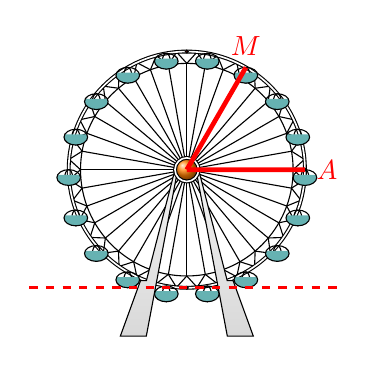
\begin{tikzpicture}[scale=.5]
		\def\r{3} 
		 \def\a{\r/10}
		 \def\n{36}
		\def\m{18} 
		 \pgfmathsetmacro{\g}{20}
		\pgfmathsetmacro{\b}{2*\a/3} 
		 \pgfmathsetmacro{\xo}{\a *cos (\g)}
		\pgfmathsetmacro{\yo}{\b  *sin (\g)}
		 \def\longdq (#1:#2){
		\begin{scope}[shift={(#1:#2)}]
			\draw (0,-\b) ellipse ({\b/2}  and {\b});
			\fill[teal!60] (\xo,\yo-\b) arc (\g:-180-\g:{\a} and {\b})--cycle; 
			 \draw (0,-\b) ellipse ({\a} and {\b});
		\end{scope}
		 }
		\foreach  \i in {1,...,\n}{
			 \pgfmathsetmacro{\gm}{360*\i/\n}
			\pgfmathsetmacro{\gh}{(360*\i+180)/\n} 
			 \pgfmathsetmacro{\gb}{360*(\i+1)/\n}
			\draw  (\gm:\r-\a)--(\gh:\r)--(\gb:\r-\a);
			\draw  (\gm:\r-\a)--(\gm:\a);
		} 
		\pgfmathsetmacro{\c}{cos (-840)}; 
		\pgfmathsetmacro{\d}{sin (-840)}; 
		\draw[double] (0:0) circle (\r); 
		\draw (0:0)  circle (\r-\a);
		 \foreach \i in {1,...,\m}{\longdq (360*\i/\m:\r)}
		\draw[top color =gray!10,bottom  color=gray!30] (-30:\a) arc (-30:0:\a) --(-70:\r)--++(\a/2,0)--([turn]-70:\r/2) --([turn]-110:2.2*\a)--(-30:\a);
		\draw[top color =gray!10,bottom color=gray!30,xscale=-1] (-30:\a)  arc (-30:0:\a) --(-70:\r)--++(\a/2,0)--([turn]-70:\r/2) --([turn]-110:2.2*\a)--(-30:\a);
		\fill[ball  color=orange] (0:0) circle (\a);
		\draw[double]  (0:0) circle (\a);
		\foreach \diem/\hoanh/\tung in {O/0/0,A/\r/0,B/\r*\c/\r*\d,C/0/\r,H/0/\r*\d,I/0/-1.42*\r,K/0/-\r} \coordinate  (\diem) at (\hoanh,\tung);
		\foreach \x in {A,K,C}{\draw[fill=red]  (\x) circle (1pt);}
		\draw[line width=1.7,red] (0,0)--(3,0) node[right]{$A$} 
			(0,0)--(60:3)  node[above]{$M$};
		 \draw[red,dashed,line width=1.2] (-4,-3)--(4,-3);
	\end{tikzpicture}
	} 
	 \shortans{10}
	 \loigiai{
		Ta có $h(x)=4+4\sin  \alpha$.\\
		Khi $M$ ở vị trí cao nhất so với mặt nước (tức là  $h(x)=8$) thì $\sin \alpha=1\Rightarrow \alpha=\dfrac{\pi}{2}$ (vì chỉ xét $1$ vòng quay đầu tiên).\\
		Thời gian thực hiện của  guồng nước là $t=\dfrac{\dfrac{\pi}{2} \cdot 40}{2\pi}=10$ (giây).
	 }
\end{ex}

% nguồn: Ok_TraLoiNgan_Lop11_Lan1
\begin{ex}%[1D1V5-6]%[ma:2d35987c]
	Số giờ có ánh sáng mặt trời của một thành phố $A$ ở vĩ độ $40^{\circ}$ bắc trong ngày thứ $t$ của một năm  không nhuận được cho bởi hàm số
	 $$
	d(t)=3\sin \left[\frac{\pi}{182}(t-80)\right]+12 \text { với } t \in  \mathbb{Z} \text { và } 0<t \leq 365.
	 $$
	Vào ngày nào trong năm thì thành phố $A$ có nhiều giờ có ánh sáng mặt  trời nhất?
	 \shortans{171}
	 \loigiai{
		Thành phố $A$ có nhiều giờ có ánh sáng mặt  trời nhất đồng nghĩa với $d(t)$ lớn nhất. Điều này xảy ra khi
		\begin{eqnarray*}
			 &&\sin \left[\dfrac{\pi}{182}(t-80)\right]=1\\
			&\Leftrightarrow& \dfrac{\pi}{182}(t-80)=\dfrac{\pi}{2}+k  2\pi\\
			 &\Leftrightarrow& t=80+91+k364\\
			&\Leftrightarrow& t=171+364k\\ 
			&\Leftrightarrow &  t=171 \text{ (do $0<t \leq 365$).}
		\end{eqnarray*}
	} 
\end{ex}

% nguồn: Ok_TraLoiNgan_Lop11_Lan1
\begin{ex}%[1D1V5-6]%[ma:d0f3fce0]
	Hằng ngày mực nước của con kênh lên xuống theo thủy triều. Độ sâu $h$ m của mực nước trong kênh tính theo thời gian  $t \text{(giờ)}(0 \leq t \leq 24)$ được cho bởi công thức $h(t)=3 \cos \left(\dfrac{\pi t}{12}+\dfrac{\pi}{4}\right)+14$. Thời điểm (giờ) nào trong ngày mực nước trong kênh là cao nhất?
	 \shortans{21}
	\loigiai{Ta có \\ 
		$-3 \leq 3 \cos \left(\dfrac{\pi t}{12}+\dfrac{\pi}{4}\right) \leq 3 \Leftrightarrow 11  \leq 3 \cos \left(\dfrac{\pi t}{12}+\dfrac{\pi}{4}\right)+14 \leq 17 \Leftrightarrow 11 \leq h \leq 17$.\\
		Khi đó $\operatorname{Max}  h=17 \Leftrightarrow \cos \left(\dfrac{\pi t}{12}+\dfrac{\pi}{4}\right)=1 \Leftrightarrow \dfrac{\pi t}{12}+\dfrac{\pi}{4}=k 2 \pi \Leftrightarrow t=-3+24 k(k \in \mathbb{Z}).$\\
		Mà $\heva{ &  t \in \mathbb{N} \\ & 0 \leq t \leq 24}$ nên $k=1 \Rightarrow t=-3+24\cdot1=21$h.\\
	Vậy thời điểm mực nước trong kênh cao nhất trong ngày là  $21$h.}
\end{ex}

% nguồn: Ok_TraLoiNgan_Lop11_Lan1
\begin{ex}%[1D1V5-6]%[ma:5c6b7c07]
	Nhiệt độ ngoài trời ở một thành phố vào các thời điểm khác nhau trong ngày có thể được mô phỏng bởi công thức $h(t)=29+3\sin \left[\dfrac{\pi}{12}(t-9)\right]$ với $h$ tính bằng  độ $\mathrm{C}$ và $t$ là thời gian trong ngày tính bằng giờ. Nhiệt độ thấp nhất trong ngày là vào lúc mấy giờ?
	\shortans{3} 
	\loigiai{ 
		Ta có $$-1\leq \sin \left[\dfrac{\pi}{12}(t-9)\right]\leq 1\Leftrightarrow 26 \leq 29+3\sin \left[\dfrac{\pi}{12}(t-9)\right]\leq  32\ (\forall t\geq 0).$$
		Vậy nhiệt  độ thấp nhất trong ngày là $26^{\circ}\mathrm{C}$, xảy ra khi
		$$\sin \left[\dfrac{\pi}{12}(t-9)\right]=-1 \Leftrightarrow \dfrac{\pi}{12}(t-9)=-\dfrac{\pi}{2}+k2\pi \Leftrightarrow  t=3+24k,k \in \mathbb{Z}.$$
		Do $t$ là thời gian trong ngày  tính bằng giờ nên $0 \leq t \leq 24$.\\
		Suy ra  $t=3$.
	} 
\end{ex}

% nguồn: Ok_TraLoiNgan_Lop11_Lan1
\begin{ex}%[1D1V5-6]%[ma:db05e891]
	Số giờ có ánh sáng mặt trời  của một thành phố A trong ngày thứ $t$ của năm $2017$ được cho bởi một hàm số $y=4\sin \left[\dfrac{\pi}{178}\left(t-60\right)\right]+10$ với $t\in \mathbb{Z}$ và $0<t\le 365$. Vào ngày thứ bao nhiêu trong năm thì thành phố $A$ có nhiều giờ có ánh sáng mặt trời nhất?
	\shortans{149} 
	\loigiai{ 
		Vì $\sin \left[\dfrac{\pi}{178}\left(t-60\right)\right]\le 1\Rightarrow y=4\sin \left[\dfrac{\pi}{178}\left(t-60\right)\right]+10\le  14$.\\
		Ngày có ánh sáng mặt  trời nhiều nhất \[\Leftrightarrow y=14\Leftrightarrow \sin \left[\dfrac{\pi}{178}\left(t-60\right)\right]=1
		\Leftrightarrow  \dfrac{\pi}{178}\left(t-60\right)=\dfrac{\pi}{2}+k2\pi \Leftrightarrow t=149+356k.\]
		Do  $0<t\le 365\Rightarrow0<149+356k\le 365\Leftrightarrow -\dfrac{149}{356}<k\le \dfrac{54}{89}\xrightarrow{k\in \mathbb{Z}}k=0$.\\
	Với $k=0 \Rightarrow  t=149$.}
\end{ex}

% nguồn: Ok_TraLoiNgan_Lop11_Lan1
\begin{ex}%[1D1V5-6]%[ma:86ff0902]
	\immini{Một vật nặng treo bởi một chiếc lò xo, chuyển động lên xuống qua vị trí cân bằng. Khoảng cách $h$ từ vật đến vị trí cân bằng ở thời điểm $t$ giây được tính theo công thức $h=|d|$ trong đó $d=5\sin 6t-4\cos 6t$ với $d$ được tính bằng centimet.  Hỏi trong giây đầu tiên, có bao nhiêu thời điểm vật ở xa vị trí cân bằng nhất?\\
	 \shortans{2}
	}{\begin{tikzpicture}[scale=.75,font=\footnotesize,line join=round,line cap=round,>=stealth]
		\node[rectangle,draw,minimum width=8mm,minimum height =  6mm] (a) at (0,2) {};
		 \node[rectangle,draw,fill=blue,minimum width=8mm,minimum height = 6mm] (b) at (0,0) {};
		\draw[decoration={aspect=0.3,segment  length=1.5mm,amplitude=3mm,coil},decorate] (0,5) -- (a);
		\draw[dashed,decoration={aspect=0.3,segment length=3mm,amplitude=3mm,coil},decorate] (0,2.25) --  (b);
		\fill [pattern = north east lines] (-1,5) rectangle (1.3,5.2); 
		\draw (-1,5)  -- (1.3,5);
		\draw (-3.5,1)--(1,1); 
		\draw (-3.5,1)--(1,1); 
		 \node () at (-2.4,1.2){V{ị} tr{í} c{â}n b{ằ}ng};
		\draw  (0.4,2)--(1,2);
		\draw[<->] (0.6,1)--(0.6,2) node[midway,right]{$h$}; 
	\end{tikzpicture}
	 }
	 \loigiai{
		Ta có \\$h=|d|=|5\sin 6t-4\cos  6t|=\sqrt{41}\left|\dfrac 5{\sqrt{41}}\sin 6t-\dfrac 4{\sqrt{41}}\cos 6t\right|=\sqrt{41}|\sin(6t-\alpha)|\leqslant\sqrt{41}$.\\
		Với $\heva{&\cos\alpha=\dfrac 5{\sqrt{41}}\\ &\sin\alpha=\dfrac  4{\sqrt{41}}.}$\\
		Vật  ở xa vị trí cân bằng nhất nghĩa là
		$\begin{aligned}
		h_{\max}=\sqrt{41} 
		&\Leftrightarrow|\sin(6t-\alpha)|=1\\ 
		 &\Leftrightarrow \cos(6t-\alpha)=0\\
		 &\Leftrightarrow 6t-\alpha=\dfrac{\pi}2+k\pi\\
		 &\Leftrightarrow t=\dfrac{\alpha}6+\dfrac{\pi}{12}+k\dfrac{\pi}6.
	\end{aligned}$\\
	\noindent Trong  giây đầu tiên nên
	$\begin{aligned}
	 0\leqslant t\leqslant 1
	&\Leftrightarrow 0\leqslant \dfrac{\alpha}6+\dfrac{\pi}{12}+k\dfrac{\pi}6\leqslant 1\\ 
	&\Leftrightarrow -\dfrac{\alpha}{\pi}-\dfrac  12\leqslant k\leqslant\dfrac 6{\pi}-\dfrac{\alpha}{\pi}-\dfrac 12\\
	 &\Leftrightarrow k\in\{0; 1\}.
	\end{aligned}$\\
	Vậy có hai lần vật ở xa vị trí  cân bằng nhất.
} 
\end{ex}

% nguồn: Ok_TraLoiNgan_Lop11_Lan1
\begin{ex}%[1D1V5-6]%[ma:f6565c29]
	Một quả đạn pháo được bắn khỏi nòng pháo với vận tốc ban đầu $v_0$ m/s hợp với phương ngang một góc $\alpha $. Ta biết rằng, nếu bỏ qua sức cản của không khí và coi quả đạn pháo được bắn  ra từ mặt đất thì quỹ đạo của quả đạn tuân theo phương trình $y=\dfrac{-g}{2v_0^2\cos^2\alpha }{x^2}+x\tan\alpha $, ở đó $g=9{,}8$ m/s$^2$ là gia tốc trọng trường. Biết quả đạn có tầm bắn xa nhất theo phương ngang $x_{\max}=9183{,}7$ (m), khi đó $v_0$ bằng bao nhiêu (kết quả làm tròn đến hàng đơn vị).
	 \shortans{300}
	\loigiai{ 
		Chọn hệ trục tọa độ có gốc tọa độ đặt tại vị trí khẩu pháo, trục $Ox$ theo phương ngang và chiều dương trùng với hướng khẩu pháo.\\ 
		\begin{center}
			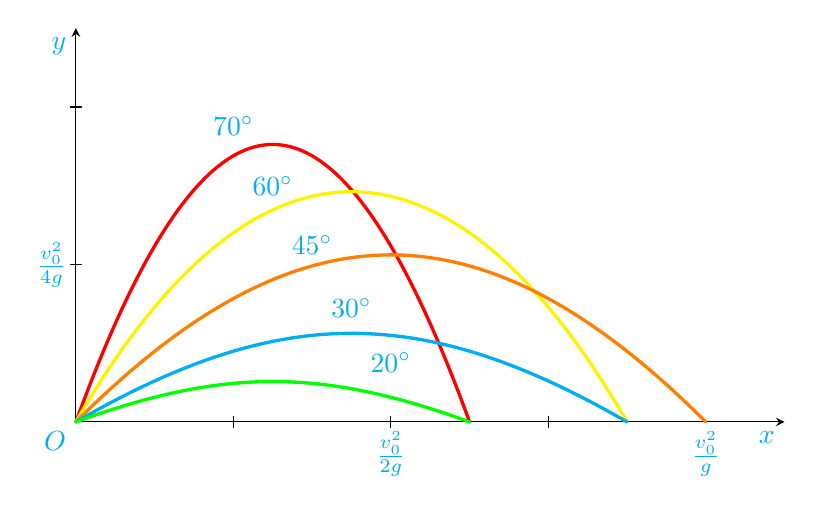
\begin{tikzpicture}[line join=round,line cap=round,>=stealth]
					\draw[-stealth] (0,0)  -- (9,0) node[cyan,below left]{$x$};
					 \draw[-stealth] (0,0) -- (0,5) node[cyan,below left]{$y$};
					\foreach \x  in {2,4,6}
					\draw  [shift={(\x,0)},color=black] (0pt,2pt)--(0pt,-2pt);
					\foreach  \y in {2,4}
					\draw  [shift={(0,\y)},color=black] (2pt,0pt)--(-2pt,0pt);
					\draw[red,very  thick] (0,0).. controls +(70:5) and +(110:5).. (5,0);
					\draw[yellow,very thick] (0,0).. controls +(60:4.5) and +(120:4.5).. (7,0); 
					\draw[orange,very thick]  (0,0).. controls +(45:4) and +(135:4).. (8,0);
					\draw[cyan,very thick] (0,0).. controls +(30:3) and  +(150:3).. (7,0);
					\draw[green,very thick] (0,0).. controls +(20:2) and +(160:2).. (5,0); 
					\draw[cyan] 
						(0,0) node[below left]{$O$} 
						(0,2)  node[left]{$\frac{v_{0}^{2}}{4g}$}
						(4,0) node[below]{$\frac{v_{0}^{2}}{2g}$} 
						(8,0) node[below]{$\frac{v_{0}^{2}}{g}$} 
						(2,4) node[below] {$70^\circ$} 
						(2.5,3)  node {$60^\circ$}
						(3,2) node[above]  {$45^\circ$}
						(3.5,1.2) node[above] {$30^\circ$} 
						(4,1) node[below]  {$20^\circ$};
				\end{tikzpicture}
		\end{center}
		Ta biết rằng quỹ đạo của quả đạn pháo có dạng đường parabol có phương trình \\$y=\dfrac{-g}{2v_0^2\cdot \cos^2\alpha}{x^2}+x\cdot\tan\alpha $, ở đó $g=9{,}8$ m/s$^2$ là gia tốc trọng  trường.\\
		Quả đạn chạm đất khi $y=0\Leftrightarrow \dfrac{-g}{2v_0^2\cos^2\alpha }{x^2}+x\tan\alpha =0$ $\Leftrightarrow$ 
		$\hoac{& x=0 \\ 
		& x=\dfrac{v_0^2\sin  2\alpha }{g}}$.\\
		Do đó quả đạn tiếp  đất khi $x=\dfrac{v_0^2\sin 2\alpha }{g}$.\\
		Ta có $x=\dfrac{v_0^2\sin 2\alpha }{g}\le \dfrac{v_0^2}{g}$, đẳng thức xảy  ra khi $\sin 2\alpha =1$ hay $\alpha =45{}^\circ $.\\
		 Suy ra quả đạn có tầm bắn xa nhất theo phương ngang là ${x_{\max }}=\dfrac{v_0^2}{g}=9183{,}7$.\\
		 $v_0^2 = 9183{,}7\cdot 9{,}8 = 90000{,}26$.\\
		Do đó $v_0\approx 300$ (m/s). 
	} 
\end{ex}

% nguồn: Ok_TraLoiNgan_Lop11_Lan1
\begin{ex}%[1D1V5-6]%[ma:16807dfe]
	Một quả đạn pháo được bắn ra khỏi nòng pháo với vận tốc ban đầu $ v_0=500$ m/s hợp với phương ngang một góc $ \alpha $. Trong Vật lí, ta biết rằng, nếu bỏ qua sức cản của không khí và coi quả đạn pháo được bắn ra từ mặt đất thì quỹ đạo của quả đạn  tuân theo phương trình $ y=\dfrac{-g}{2v_0^2\cos^2\alpha}\cdot x^2+x\tan \alpha $, trong đó $g = 10$ m/s$ ^2 $ là gia tốc trọng trường. Góc bắn $ \alpha $ để quả đạn bay xa nhất là bao nhiêu độ?
	 \shortans{45}
	 \loigiai{
		Ta có \begin{eqnarray*}
		y=0&\Leftrightarrow& \dfrac{-g}{2v_0^2\cos^2\alpha}\cdot x^2+x\tan  \alpha=0\\
		&\Leftrightarrow & x\left(\dfrac{-g}{2v_0^2\cos^2\alpha}\cdot  x+\tan \alpha \right)=0 \\
		&\Leftrightarrow & \hoac{&x=0\\&x=\dfrac{v_0^2\sin2\alpha}{g}= 25~000\sin2\alpha.} 
	\end{eqnarray*}
	Vậy tầm bay xa mà quả  đạn đạt tới là $25~000\sin2\alpha$ m.\\
	 Vậy đạn bay xa nhất khi $ \sin2\alpha=1\Leftrightarrow 2\alpha=\dfrac{\pi}{2}+k2\pi\Leftrightarrow \alpha =\dfrac{\pi}{4}+k\pi $.\\
	Vì $ 0\le\alpha\le  \dfrac{\pi}{2} $ nên $ \alpha=\dfrac{\pi}{4} $.\\
	Vậy góc bắn  bằng $ 45^\circ $ thì đạn bay xa nhất.
 }
\end{ex}

% nguồn: Ok_TraLoiNgan_Lop11_Lan1
\begin{ex}%[1D1V5-6]%[ma:5ac086bb]
	 \immini[thm]{
	Hội Lim (tỉnh Bắc Ninh) vào mùa xuân thường có trò chơi đánh đu. Khi người chơi đu nhún đều, cây đu sẽ đưa người chơi đu dao động qua lại vị trí  cân bằng (\textit{tham khảo hình vẽ bên}). Nghiên cứu trò chơi này, người ta thấy khoảng cách $h$ (m) từ người chơi đu đến vị trí cân bằng được biểu diễn qua thời gian $t$ (s) (với $t\ge 0$) bởi hệ thức $h=|d|$ với $d=3\cos\left[\dfrac{\pi}{3}(2t-1)\right]$, trong đó quy ước $d>0$ khi vị trí cân bằng ở phía sau lưng người chơi đu và $d<0$ trong trường hợp ngược lại (\textit{Nguồn: R.Larson and B.Edwards, Calculus 10e Cengage}). Tìm thời điểm đầu tiên mà khoảng cách $h$ lớn nhất. (Viết kết quả dưới dạng số thập phân).
	 }
	{\definecolor{darkpastelgreen}{rgb}{0.01, 0.75,  0.24}
	\definecolor{almond}{rgb}{0.94,  0.87, 0.8}
	\definecolor{arsenic}{rgb}{0.23, 0.27, 0.29} 
	 \definecolor{eggplant}{rgb}{0.38, 0.25, 0.32}
	\definecolor{crimson}{rgb}{0.86, 0.08,  0.24}
	\begin{tikzpicture}[line join=round,line cap=round,scale=0.8,transform shape]
			\clip  (-2.5,-2.5) rectangle (4.5,4.2);
			\tikzset{q_h/.pic={ 
			\draw[fill=darkpastelgreen] (-.05,4)--(.9,-1.8) 
				..controls +(30:.05) and +(-30:.05)..(1,-1.75)--(.05,4); 
			 \draw[fill=darkpastelgreen] (-.1,4)--(.6,-1.4)
				..controls +(30:.05) and  +(-30:.05)..(.5,-1.4)--(-.2,4);
			 \def\M{
				(-.2,1.76) 
				 ..controls +(-80:.1) and +(80:.1)..(-.18,1.6)
				..controls +(-40:.1)  and +(30:.06)..(-.18,1.5)--(-.17,1.46)--(-.22,1.44)--(-.19,1.43)--(-.2,1.43)
				..controls +(-80:.1) and  +(-12:.05)..(-.3,1.35)--(-.35,1.28)--(-.55,1.35)
				..controls +(60:.1) and  +(-90:.05)..(-.45,1.5)
				 ..controls +(100:.1) and +(140:.05)..(-.38,1.55)
				..controls  +(70:.1) and +(-140:.05)..cycle;
			 }
			\draw[black]\M; 
			\fill[almond]  \M;
			\draw (-.2,1.76) 
				 ..controls +(-140:.1) and +(50:.05)..(-.3,1.6)
				(-.2,1.76) 
				..controls  +(-120:.1) and +(40:.05)..(-.25,1.6)
				(-.28,1.578) 
				..controls +(-20:.02) and  +(-150:.02)..(-.22,1.58)
				(-.25,1.568)--(-.23,1.567); 
			 \def\A3{
				(-.1,.9) 
				..controls  +(-30:.05) and +(110:0)..(.18,1)
				 --(.19,.95)
				..controls +(-140:.05) and +(30:.05)..(-.1,.7)--cycle; 
			} 
			\fill[arsenic]  \A3;
			 \draw[black]\A3;
			 \def\A2{
				 (-.35,1.28)
				..controls +(-30:.05) and +(110:.05)..(-.25,1.18) 
				 ..controls +(-70:.05) and +(90:.02)..(-.05,.9)
				..controls +(-90:.02)  and +(50:.05)..(-.05,.4)
				..controls  +(-130:.02) and +(50:.05)..(.6,-.8)
				 ..controls +(-130:.02) and +(50:.05)..(.9,-1.8)
				..controls +(-130:.2) and  +(30:.3)..(-.5,-2.3)
				..controls +(130:.2) and +(-90:.1)..(-.2,-1.5) 
				 ..controls +(130:.2) and +(-140:.1)..cycle;
			 }
			 \fill[arsenic] \A2;
			 \draw[black]\A2;
			 \def\A{
				 (-.55,1.35)
				 ..controls +(-150:.2) and +(120:.1)..(-.45,0)
				..controls +(-60:.1) and  +(50:.1)..(-.3,-1.6)
				..controls  +(-10:.1) and +(-120:.1)..(-.15,-1.5)
				..controls +(60:.1) and +(-120:.1)..(0,-1.45) 
				..controls +(120:.3) and  +(-50:.1)..(-.35,.77)
				..controls +(-50:.1) and +(130:.1)..(-.15,.48) 
				..controls  +(-50:.1) and +(-130:.1)..(.43,.93)
				..controls  +(-130:.05) and +(-40:.05)..(.3,1.05)
				..controls +(-130:.05) and  +(40:.05)..(-.05,.75)
				..controls +(-140:.05) and  +(-40:.05)..(-.3,1.15)
				..controls +(100:.05) and +(-40:.05)..(-.35,1.28)--cycle; 
			 }
			\fill[eggplant]  \A;
			\draw[black]\A; 
			 \def\N{
				(-.14,1.95) 
				 ..controls +(-80:.1) and +(80:.1)..(-.17,1.7)
				..controls  +(110:.02) and +(-40:.02)..(-.2,1.76)
				..controls  +(-110:.1) and +(50:.4)..(-.48,1.45)--(-.45,1.35)..controls +(-150:.05) and +(20:.05)..(-.7,1.32)
				 ..controls +(50:.05) and +(-120:.05)..(-.65,1.45)
				..controls +(160:.02) and +(-50:.02)..(-.7,1.48) 
				..controls  +(160:.02) and +(-50:.02)..(-.8,1.6)--(-.75,1.63)
				 ..controls +(-20:.06) and +(130:.04)..(-.6,1.47)
				..controls  +(130:.2) and +(-90:.1)..(-.7,1.78)
				 ..controls +(90:.1) and +(170:.1)..(-.4,1.9)
				..controls +(20:.1) and  +(160:.1)..cycle;
			 }
			\fill[arsenic] \N; 
			\draw[black]\N; 
			\draw (-.14,1.95) 
				..controls +(-100:.05) and +(40:.06)..(-.2,1.76) 
				(-.5,1.55) 
				..controls +(30:.1) and  +(-100:.06)..(-.3,1.76)
				(-.6,1.7) 
				 ..controls +(-55:.1) and +(120:.06)..(-.55,1.5);
			 \def\T1{
				 (.3,1.03)
				 ..controls +(60:.05) and +(-120:.05)..(.35,1.15)
				 ..controls +(60:.05) and +(-140:.05)..(.45,1.26)
				..controls +(30:.05) and +(60:.04)..(.5,1.22) 
				..controls +(30:.03) and +(50:.03)..(.54,1.18) 
				..controls +(30:.03) and  +(50:.03)..(.56,1.12)
				 ..controls +(30:.03) and +(50:.03)..(.58,1.07)
				..controls +(160:.03) and +(40:.03)..(.49,1) 
				..controls  +(-140:.03) and +(40:.03)..(.41,.92)--cycle;
			 }
			 \fill[almond] \T1;
			\draw[black]\T1; 
			\fill[crimson](-.27,.4) 
				..controls +(-80:.6) and +(-80:.1)..(-.5,-1.9)--(-.45,-1.85) 
				..controls +(90:.1) and  +(-80:1)..(-.28,.48)--cycle;
			 \fill[crimson](-.27,.4)
				..controls +(-80:.6)  and +(-80:.1)..(-.2,-1.9)--(-.15,-1.85)
				 ..controls +(90:.1) and +(-80:1)..(-.28,.48)--cycle;
				 }}
			 \tikzset{no/.pic={
			\draw[crimson] (1.8,-1) 
				 ..controls +(150:.4) and +(-120:.5)..(1.7,-1)
				..controls +(30:.4) and  +(-40:.3)..(1.75,-1)
				..controls +(-30:.2)  and +(40:.2)..(1.7,-1.4)
				 (1.75,-1)
				..controls  +(-50:.1) and +(20:.1)..(1.7,-1.2);
				}} 
			\draw (4,-1.25) arc  (-60:-120:6cm);
			 \draw[dashed] (4,-1.25)--(1.3,4)--(-2,-1.25)
				(1.3,4)--(1.3,-2); 
			\node at (1.5,.5) [rotate=90]{\tiny Vị trí  cân bằng};
			\draw[thick,<->] (.35,-2)--(1.3,-2); 
			 \node at (.85,-2) [above]{\tiny $h$};
			\fill (4,-1.25) circle (0.05); 
			 \fill (-2,-1.25) circle (0.05);
			\fill (1.3,4) circle (0.05); 
			 \path
				(0,0) pic[scale=1,rotate=-20]{q_h} 
				 (-.88,1.48) pic[scale=1,scale=.7,rotate=-20]{no};
		\end{tikzpicture}
	} 
	\shortans{0,5} 
	\loigiai{ 
		Do $-1 \leq \cos \left[\dfrac{\pi}{3}(2 t-1)\right] \leq 1$  nên $-3 \leq 3 \cos \left[\dfrac{\pi}{3}(2 t-1)\right] \leq 3$ hay $-3 \leq d \leq 3$.\\
		Do đó, $0 \leq|d| \leq 3$. Vậy $h$ lớn nhất bằng 3  khi $|d|=3$ hay
		\begin{eqnarray*}
			 && \cos\left[\dfrac{\pi}{3}(2 t-1)\right]= \pm 1\\
			&\Leftrightarrow& \sin  \left[\dfrac{\pi}{3}(2 t-1)\right]=0 \\
			 & \Leftrightarrow& \dfrac{\pi}{3}(2 t-1)=k \pi\\
			&\Leftrightarrow& t=\dfrac{1+3 k}{2}  \text { với } k \in \mathbb{N}.
		\end{eqnarray*}
		Thời điểm đầu tiên mà khoång cách $h$ lớn nhất là  $t=0{,}5$ s (ứng với $k=0$).
	 }
\end{ex}

% nguồn: Ok_TraLoiNgan_Lop11_Lan1
\begin{ex}%[1D1V5-6]%[ma:40a7f74e]
	Một cây cầu có dạng cung $OM$ của đồ thị hàm số $y = 2{,}1 \sin \dfrac{x}{10}$ và được mô tả trong hệ trục  tọa độ với đơn vị trục là mét như hình vẽ dưới đây
	\begin{center}
		\begin{tikzpicture}[>=stealth,scale=0.8]
				\draw[->,line width = 1pt]  (-1,0)--(0,0)
					 node[below right]{$O$}--(15,0) node[below]{$x$};
				\draw[->,line width = 1pt]  (0,-0.5) --(0,3) node[right]{$y$};
				\draw [smooth,samples=100,domain=0:12.5,font=\footnotesize,line join=round,line cap=round]  plot (\x,{2.1*sin ((\x/4)*180/pi)});
				 \draw (12.5,0) node[below]{$M$};
			\end{tikzpicture}
	\end{center}
	Giả sử chiều rộng của con sông là độ dài đoạn thẳng $OM$. Tìm chiều  rộng đó (làm tròn kết quả đến hàng phần mười).
	 \shortans{31,4}
	\loigiai{ 
		Ta có  hai vị trí $O$ và $M$ là hai vị trí chân cầu, tại hai vị trí này ta có $y=0$.\\
		Khi đó ta có $\sin \dfrac{x}{10} = 0  \Leftrightarrow \dfrac{x}{10} = k\pi \Leftrightarrow x=9k\pi \quad(k \in \mathbb{Z})$.\\
		Quan sát đồ thị ở trên, ta thấy đồ  thị cắt trục hoành tại hai điểm $O$ và $M$ liên tiếp nhau với $x \geq 0$.\\
		Xét với $k=0$ ta có $x=0$.\\ 
		Xét với $k=1$  ta có $x=10\pi$.\\
		Mà $x=0$ là hoành độ của điểm $O$ nên hoành độ của điểm $M$  là $x=10\pi$.\\
		Vậy chiều rộng cần tìm là $OM =  10\pi \approx 31{,}4$.
	} 
\end{ex}

% nguồn: Ok_TraLoiNgan_Lop11_Lan1
\begin{ex}%[1D1V5-6]%[ma:64188c2b]
	Một chiếc lò xo một đầu cố định, một đầu gắn chất điểm $A$. Nén lò xo một  lực làm chất điểm $A$ dao động xung quanh vị $O$, quãng đường chất điểm $A$ di chuyển được xác định bởi công thức $s=2\sin\left(2t+\dfrac{\pi}{4}\right)$ (cm), với $t$ là thời gian được tính bằng giây~(s). Trong $3$ giây đầu, thời điểm nào thì $s = \sqrt{3}$ (cm) (Làm tròn kết quả đến hàng phần trăm)?
	\shortans{0,13} 
	\loigiai{ 
		 Ta có\\
		\begin{align*}
			&2\sin\left(2t+\dfrac{\pi}{4}\right) =  \sqrt{3} \\
			\Leftrightarrow &\sin \left(2t+\dfrac{\pi}{4}\right) = \dfrac{\sqrt{3}}{2} = \sin\left(\dfrac{\pi}{3}\right)\\ \Leftrightarrow &\hoac{&2t  + \dfrac{\pi}{4} = \dfrac{\pi}{3} + k2\pi\\&2t + \dfrac{\pi}{4} = \pi - \dfrac{\pi}{3} + k2\pi\\} \\
			 \Leftrightarrow &\hoac{&t = \dfrac{\pi}{24} + k\pi\\&t=\dfrac{5\pi}{24} + k\pi}\quad k \in \mathbb{Z}.\\
		\end{align*}
		Với $0<t\le 3$, ta chọn $t=\dfrac{\pi}{24}\approx 0{,}13$ với  $k=0$.
	} 
\end{ex}

% nguồn: Ok_TraLoiNgan_Lop11_Lan1
\begin{ex}%[1D1V5-6]%[ma:0c6f3ddd]
	Cho hai vật dao động điều hòa theo phương trình lần lượt là $x_1(t)=8\cos\left(4\pi  t+\dfrac{\pi}{2}\right)$ $(\mathrm{cm})$ và $x_2(t)=-8\cos (4\pi t)$ $(\mathrm{cm})$, trong đó $x_1(t)$, $x_2(t)$ là li độ của hai vật tại thời điểm $t$ (giây). Khi hai vật dao động trong thời gian từ $0$ đến $10$ giây, hỏi chúng có cùng li độ mấy lần?
	 \shortans{40}
	 \loigiai{
		Thời điểm hai vật có cùng li độ, ta có  $8\cos\left(4\pi t+\dfrac{\pi}{2}\right)=-8\cos (4\pi t)$
		$$\begin{aligned}
		 &\Leftrightarrow
		\cos\left(4\pi t+\dfrac{\pi}{2}\right)=\cos (\pi-4\pi  t)\\
		& \Leftrightarrow \hoac{&4\pi t+\dfrac{\pi}{2}=\pi-4\pi t+k2\pi\\&4\pi  t+\dfrac{\pi}{2}=-\pi+4\pi t+k2\pi}\\
		& \Leftrightarrow \hoac{&8\pi t=\dfrac{\pi}{2}+k2\pi\\&0t=-\dfrac{3\pi}{2}+k2\pi\text{: vô  nghiệm}}\\
		 & \Leftrightarrow
		t=\dfrac{1}{16}+\dfrac{k}{4} \  (k \in \mathbb{Z}).
	\end{aligned}$$
	Xét $t \in [0;10]$,  ta có $0 \leq \dfrac{1}{16}+\dfrac{k}{4} \leq 10 \Leftrightarrow -\dfrac{1}{4} \leq k \leq \dfrac{159}{4} \Leftrightarrow k \in \{0;1;2;\ldots;39\}$ (do $k \in \mathbb{Z}$).\\
	Vậy trong $10$ giây  đầu tiên, hai vật có cùng li độ $40$ lần.
} 
\end{ex}

% nguồn: Ok_TraLoiNgan_Lop11_Lan1
\begin{ex}%[1D1V5-6]%[ma:50064541]
	Hằng ngày mực nước con kênh lên xuống theo thủy triều. Độ sâu $h$ (mét) của mực nước trong kênh được tính tại thời điểm $t$ (giờ) trong một ngày bởi công thức $h=3 \cos \left(\dfrac{\pi t}{4}-5 \pi\right)+5$. Hỏi thời điểm  nào trong ngày mực nước trong kênh đạt độ cao $h=8$ (mét).
	\shortans{20} 
	 \loigiai{
	 Mực nước trong kênh cao $8$ m, nghĩa là
	 {\allowdisplaybreaks
	\begin{eqnarray*}
		&&  3 \cos \left(\dfrac{\pi t}{4}-5 \pi\right)+5=8 \\
		& \Leftrightarrow & \dfrac{\pi t}{4}-5 \pi= 1\\ 
		& \Leftrightarrow & \dfrac{\pi  t}{4}-5=k2\pi\\
		&  \Leftrightarrow & t=20+8 k.
	\end{eqnarray*}}
	Theo  yêu cầu bài toán, ta có $t=20$ (giờ).
	 }
\end{ex}

% nguồn: Ok_TraLoiNgan_Lop11_Lan2
\begin{ex}%[1D1V5-6]%[ma:6a042002]
	Hằng ngày, Mặt Trời chiếu sáng, bóng của một toà chung cư cao $40$ m intrên  mặt đất, độ dài bóng của toà nhà này được tính bằng công thức
	 $$S(t)=40\left|\cot\dfrac{\pi}{12}t\right|,$$
	với $S$ được tính bằng mét, còn $t$ là số giờ tính từ $6$ giờ sáng. Tại thời điểm nào vào buổi sáng trong ngày thì độ dài bóng của toà nhà bằng  chiều cao toà nhà?
	\shortans{9} 
	 \loigiai{
		Độ dài  bóng của toà nhà bằng chiều cao toà nhà khi $$S(t)=40\Leftrightarrow 40\left|\cot\dfrac{\pi}{12}t\right|=40\Leftrightarrow\cot\dfrac{\pi}{12}t=\pm 1\Leftrightarrow\dfrac{\pi}{12}t=\pm\dfrac{\pi}{4}+k\pi\Leftrightarrow t=\pm 3+12k\,(k\in\mathbb{Z}).$$
		Vì $0\le t\le 12$ nên $t=3$ hoặc $t=9$, tức là tại thời điểm $9$  giờ sáng hoặc $3$ giờ chiều thì bóng của toà nhà dài bằng chiều cao của toà nhà.
	} 
\end{ex}

% nguồn: Ok_TraLoiNgan_Lop11_Lan2
\begin{ex}%[1D1V5-6]%[ma:2980a357]
	Số giờ có ánh sáng của thành phố $T$ ở vĩ độ $40^\circ$ bắc trong ngày thứ $t$ của một năm không nhuận được cho bởi hàm số $d(t)=3\cdot \sin \left[\dfrac{\pi}{182} (t-80) \right]+12$ với $t\in \mathbb{Z}$ và $0< t\le 365$. Bạn An muốn đi tham quan thành phố $T$ nhưng lại không thích  ánh sáng mặt trời, vậy bạn An nên chọn đi vào ngày nào trong năm để thành phố $T$ có ít giờ có ánh sáng mặt trời nhất?
	 \shortans{353}
	 \loigiai{
		 Ta có
		\[\begin{aligned}
		&&\sin  \left[\dfrac{\pi}{182} (t-80) \right]\ge-1\\
		&\Rightarrow&  3\cdot \sin \left[\dfrac{\pi}{182} (t-80) \right]\ge-3\\
		&\Rightarrow&  3\cdot \sin \left[\dfrac{\pi}{182} (t-80) \right]+12\ge 9\\
		 &\Rightarrow& d(t) \ge 9.
	\end{aligned}\]
	Vậy thành phố $T$ có ít giờ có ánh  sáng mặt trời nhất khi và chỉ khi\\
	\[\begin{aligned}
	&&\sin \left[\dfrac{\pi}{182}  (t-80) \right]=-1\\
	 &\Rightarrow& \dfrac{\pi}{182} (t-80)=-\dfrac{\pi}{2}+k2\pi\\
	&\Rightarrow&  t-80=182\left(-\dfrac{1}{2}+2k\right)\\
	&\Rightarrow&  t=364k-11, k\in \mathbb{Z}.
	\end{aligned}\]
	 Mặt khác
	\[\begin{aligned}
	&& 0\le 364k-11\le 365\\ 
	& \Rightarrow&  \frac{11}{364}\le k \le \frac{376}{364}\\
	& \Rightarrow& k=1\quad (\text{do  } k \in \mathbb{Z}) \\
	 & \Rightarrow& t=364-11=353.
	\end{aligned}\]
	Vậy thành phố $T$ có ít giờ ánh sáng  Mặt Trời nhất là $9$ giờ khi $t=353$, tức là vào ngày thứ $353$ trong~năm.
} 
\end{ex}

% nguồn: Ok_TraLoiNgan_Lop11_Lan1
\begin{ex}%[1D1C5-6]%[ma:e2f59177]
	\immini{Giả sử vật giao động  điều hòa xung quanh vị trí cân bằng theo phương trình $x=2\cos \left(5t-\dfrac{\pi}{6} \right)$. Ở đây, thời gian $t$ tính bằng giây và quãng đường $x$ tính bằng cm. Hãy cho biết trong khoảng thời gian từ $0$ đến $6$ giây, vật đi qua vị trí cân bằng bao nhiêu lần? (hình ảnh minh họa vị trí cân bằng)}
	{\resizebox{!}{5.5cm}{\begin{tikzpicture}[>=stealth, line join=round, line cap=round, font=\footnotesize]
		\tikzset{cogai/.pic={ 
				\draw  [fill=orange!30]
				(5.73,15.68) 
				 .. controls +(-0.31,-0.1) and +(-0.19,0.37) .. ++(-0.39,-0.60)
				.. controls +(-0.19,0.13) and +(0.00,0.26) ..  ++(-0.48,-0.21)
				--++(-.8,.6)--++(.34,.65)--cycle; 
				 \draw [fill=brown!20]
				 (5.42,15.69)
				..  controls +(0.58,-0.05) and +(-0.08,-0.48) .. ++(1.11,0.58)
				.. controls  +(0.19,0.08) and +(0.24,-0.53) .. ++(0.11,0.82)
				.. controls +(0.16,0.24)  and +(0.11,-0.37) .. ++(0.16,1.01)
				..  controls +(-0.63,0.24) and +(0.05,0.90) .. ++(-1.11,-0.98)
				.. controls +(-0.21,0.13) and +(0.13,0.29)  .. ++(-0.69,-0.08)
				.. controls +(-0.16,0.61) and +(0.13,1.32) .. ++(-1.16,-0.45) 
				 .. controls +(0.19,-0.40) and +(-0.77,0.03) .. ++(1.59,-0.90);
				 \fill [black] (6.6,17.5) circle (.12)
				 (6.2,17.2) circle (.12)
				; 
				\draw (6.54,16.27)--++(-.1,0); 
				\draw  [fill=brown!30!black!90]
				 (6.80,18.10)
				..  controls +(-0.63,0.24) and +(0.05,0.90) .. ++(-1.11,-0.98)
				.. controls  +(-0.21,0.13) and +(0.13,0.29) .. ++(-0.69,-0.08)
				.. controls +(-0.16,0.61) and +(0.13,1.32) .. ++(-1.16,-0.45) 
				.. controls +(-0.61,1.43) and +(-2.30,0.50)  .. ++(2.17,2.65)
				.. controls  +(0.63,-0.13) and +(0.42,0.69) .. ++(0.79,-1.14)
				 ;
				 \draw [fill=orange]
				(6.94,18.61) 
				.. controls +(-1.06,0.73)  and +(0.90,1.57) .. ++(-3.32,-1.26)
				 .. controls +(-0.47,-0.31) and +(-0.37,-0.69) .. ++(0.32,-0.26)
				 .. controls +(0.50,0.93) and +(-1.06,0.78) .. ++(2.93,1.15)
				.. controls +(.16,-.01) and +(.18,-.22) .. cycle; 
				
				\draw [fill=green] (4.87,14.87) ..  controls +(-.37,.45) and +(.53,.03) .. ++(-1.48,.71)
				.. controls +(-.74,.11) and +(.71,-.11)  .. ++(-1.69,-.21)
				.. controls +(-.5,-.05) and +(.29,-.03)  .. ++(-.53,-1.67)
				.. controls +(-.03,-2.14)  and +(-.32,.56) .. ++(1.69,-2.06)
				.. controls +(2.65,-1.08) and +(1.06,-2.54) .. cycle 
				 ;
				\draw [fill=cyan] (2.86, 11.64) .. controls +( -1.88, -0.85) and +(  1.43, 1.03) .. ++(-4.74, -3.92)
				..  controls +( -2.80, 0.48) and +( -0.87, 1.53) .. ++(-3.25, -1.11)
				.. controls +(  0.16, -0.19) and +( -1.01, 0.08) .. ++( 1.35, -0.48)
				.. controls +( -0.13, -0.58) and +(  -1.35, -0.24) .. ++( 1.83, -1.35)
				 .. controls +( 0.77, 0.19) and +( 0.77, 0.58) .. ++( 0.77, -2.09)
				.. controls  +( 0.50, -0.42) and +( -0.03, -2.35) .. ++( 2.88, 1.19)
				.. controls +( 2.96, 1.72) and  +( -1.06, -2.43) .. ++( 3.36, 5.90)
				.. controls +(.32,.26) and +(.63,-.42) ..  ++(.08,1.14)--cycle;
				\draw [fill=yellow] (5.34,15.08) .. controls  +(.63,-.82) and +(1.06,1.24) .. ++(.16,-3.52)
				.. controls +(-.45,-.66)  and +(.5,.53) .. ++(-1.01,-1.9)
				.. controls +(-.85,.05)  and +(-.21,-.101) .. ++(-.87,.9)
				.. controls  +(.56,-.56) and +(2.25,-1.38) .. ++(-.77,1.08)
				.. controls +(2.65,-1.08)  and +(1.06,-2.54) .. ++(2.01,3.23)
				..  controls +(0,.26) and +(-.19,.13) .. cycle
				; 
				 \draw [fill=yellow](4.42, 9.02)
				.. controls +(-0.79, -0.98) and +(1.67, -0.56)  .. ++(-4.23, -2.43)
				.. controls +(-0.66,  0.19) and +(-0.16, 0.56) .. ++(-1.56, -0.24)
				.. controls +(0.29, -0.29) and +(-0.45, 0.77) .. ++(1.08, -0.95) 
				.. controls +(0.19, -0.29) and +(-1.01, -0.58) .. ++(2.38, 0.74) 
				.. controls +(0.29,  -0.11) and +(-0.82, -2.75) .. ++(2.33, 2.88);
				\draw [fill=red] (1.69,  3.89)
				.. controls +( 2.96,  1.72) and +( -1.06, -2.43) .. ++( 3.36, 5.90)
				.. controls +( 0.32, 0.26) and +( 0.63, -0.42) .. ++( 0.08,  1.14)
				.. controls +( -0.98, -0.29) and  +( 4.15, 1.16) .. ++(-4.66, -6.19)
				.. controls +( -0.21, -0.11)  and +( -1.11, 0.13) .. ++( 1.22, -0.85);
				 %
				\draw [fill=pink] (-.74,.82) .. controls +(-.56,-.9) and +(-2.96,.58) .. ++(2,-1.69) 
				.. controls +(.85,.61)  and +(.63,-.63) .. ++(-1.33,1.48)--cycle;
				\draw [fill=orange!30] (-0.31, 2.31) 
				.. controls  +(-0.06, -0.38) and +(0.32, 0.53) .. ++(-0.43, -1.49)
				.. controls +(0.19, -0.21) and +(-0.21, -0.08)  .. ++(0.74, -0.21)
				.. controls +(0.21,  0.42) and +(-0.24, -0.64) .. ++(0.42, 1.64);
				\draw [line width=.1cm, blue]  (0,0)--(27,90) coordinate (I);
				\fill [brown!45] (4.42,16.19) .. controls +(-.29,-.34) and  +(1.24,-.26) .. ++(-1.32,-1.4)
				 .. controls +(-.63,.37) and +(-.06,-1.12) .. ++(.99,1.76)--cycle;
				\fill [brown!45]  (5.00, 17.04)
				.. controls +(0.05, -0.37) and +(0.58, 0.00)  .. ++(-0.61, -0.85)
				.. controls +(-0.34, 0.19) and +(-0.29, -0.32)  .. ++(-0.21, 0.85)
				.. controls +(0.24, 0.03)  and +(-0.77, 0.79) .. ++(0.82, 0.00);
		 }}
		 \def\g{35}
		\path (0,0)  coordinate (M) pic[scale=.1]{cogai} node [below=.2] {$M$}
		 (I)++(-90:1) coordinate (I')
		($(I)!(M)!(I')$) coordinate  (M')
		($(I)!1!{atan(.3)}:(M)$)  coordinate (O)
		($(I)!1!-\g:(O)$)  coordinate (A')
		($(I)!1!\g:(O)$)  coordinate (A)
		 ;
		\draw [semithick] let 
		\p1  = ($(A)-(I)$),
		 \n1 = {atan2(\y1,\x1)},
		\p2 = ($(A')-(I)$), 
		 \n2 = {atan2(\y2,\x2)}
		 in
		(I) ++(\p1) arc[start angle=\n1, end angle=\n2, radius={veclen(\p1)}];
		% 
		 \foreach \x in {A,M,A',I,O}{
			\draw [fill=brown!50!black!90] (\x) circle  (.25);
		} 
		\fill  [gray, thick, gray] (M) circle (.1) (I) circle (.1);
		\draw [thick, dash pattern=on  2pt off 2pt] (A')--(I)--(A)
		($(I)!-0.1!(O)$)--($(O)!-0.1!(I)$) node [above, pos=.5, sloped, rotate=180] {\bf vị trí cân bằng}; 
		\draw [<->] (M)--(M') node [pos=.5, fill=white, inner sep=.5pt]  {$h$};
	\end{tikzpicture}}
	} 
	 \shortans{9}
	 \loigiai{
		Khi vật ở vị trí cân  bằng thì $x=0$
		\begin{eqnarray*}
			&\Leftrightarrow& 3\cos \left(5t-\dfrac{\pi}{6}  \right)=0\Leftrightarrow \cos\left(5t-\dfrac{\pi}{6} \right)=0\\
			&\Leftrightarrow& 5t-\dfrac{\pi}{6}=\dfrac{\pi}{2}+k\pi, k\in {\bf \mathbb{Z}}\Leftrightarrow  t=\dfrac{2\pi}{15}+\dfrac{k\pi}{5}, k\in {\bf \mathbb{Z}}.
		\end{eqnarray*}
		Mà theo  giả thiết
		\begin{eqnarray*}
			0< t < 6&\Leftrightarrow& 0< \dfrac{2\pi}{15}+\dfrac{k\pi}{5} <  6\\
			 &\Leftrightarrow&-\dfrac{2}{3} < k < \dfrac{30}{\pi}-\dfrac{2}{3}\\
			k\in {\bf \mathbb{Z}}&\Rightarrow& k\in  \left\{0;1;2;3;4;5;6;7;8\right\}.
		\end{eqnarray*}
	 }
\end{ex}

% nguồn: Ok_TraLoiNgan_Lop11_Lan1
\begin{ex}%[1D1C5-6]%[ma:7c850c88]
	Một cây cầu có dạng cung $OA$ là một  phần của đồ thị hàm số $y=4{,}8 \sin \dfrac{x}{9}$ và được mô tả trong hệ trục tọa độ với đơn vị trục là mét như hình bên.
	\begin{center}
		\begin{tikzpicture}[line join=round,line cap=round,>=stealth,scale=.85,transform shape]
				\def\xmin{0}  \def\xmax{12} \def\ymin{-.5} \def\ymax{2}
				\draw[->](\xmin-.5,0)--(\xmax+1,0) node[below]{$x$}; 
				\draw[->](0,\ymin)--(0,\ymax+.5) node[left]{$y$}; 
				\draw (0,0) node[below right]{$O$}; 
				\draw  (\xmin,0) to [out=40,in= 140] (\xmax,0) node[below]{$A$};
			\end{tikzpicture}
	\end{center}
	Giả sử chiều rộng của con sông là độ  dài đoạn thẳng $OA$. Chiều rộng đó (làm tròn đến kết quả hàng phần mười) là
	\shortans{28,3} 
	\loigiai{ 
		 Phương trình hoành độ giao điểm
		$$4{,}8 \sin  \dfrac{x}{9}=0\Leftrightarrow\sin \dfrac{x}{9}=0\Leftrightarrow\dfrac{x}{9}=k\pi\Leftrightarrow x=9k\pi,\ (k\in \mathbb{Z}).$$
		Hoành độ điểm $A$ ứng  với $x=9\pi$.\\
		Vậy  $OA=9\pi\approx 28{,}3$m.
	} 
\end{ex}

% nguồn: Ok_TraLoiNgan_Lop11_Lan1
\begin{ex}%[1D1C5-6]%[ma:7136996e]
	Vận tốc $v_1$ (cm/s) của con lắc  đơn thứ nhất và vận tốc $v_2$ (cm/s) của con lắc đơn thứ hai theo thời gian $t$ (giây) được cho bởi các công thức:
	$$v_1(t)=-4 \cos \left(\dfrac{2 t}{3}+\dfrac{\pi}{4}\right) $$  và $$ v_2(t)=2 \sin \left(2 t+\dfrac{\pi}{6}\right).$$
	Hãy cho biết trong khoảng thời  gian $t\in [0;10]$, có bao nhiêu lần vận tốc của con lắc đơn thứ nhất gấp hai lần vận tốc của con lắc đơn thứ hai.\\
	\shortans{6} 
	\loigiai{Thời điểm $t$ mà tại vận tốc của con lắc đơn thứ nhất gấp hai lần vận tốc của con lắc đơn thứ hai là nghiệm của  phương trình:
		\begin{eqnarray*}
			&&-4 \cos \left(\dfrac{2 t}{3}+\dfrac{\pi}{4}\right)=2\cdot2 \sin \left(2 t+\dfrac{\pi}{6}\right) \\ 
			&\Leftrightarrow  &\cos \left(\dfrac{2 t}{3}+\dfrac{\pi}{4}\right)=-\sin \left(2 t+\dfrac{\pi}{6}\right) \\
			&\Leftrightarrow  &\cos \left(\dfrac{2 t}{3}+\dfrac{\pi}{4}\right)=\sin \left(-2 t-\dfrac{\pi}{6}\right) \\
			&\Leftrightarrow &\cos \left(\dfrac{2 t}{3}+\dfrac{\pi}{4}\right) = \cos \left[\dfrac{\pi}{2}-\left(-2 t-\dfrac{\pi}{6}\right)\right]\\ 
			&\Leftrightarrow & \cos  \left(\dfrac{2 t}{3}+\dfrac{\pi}{4}\right) = \cos \left(2 t+\dfrac{2\pi}{3}\right)\\
			 &\Leftrightarrow & \hoac{&\dfrac{2 t}{3}+\dfrac{\pi}{4}=2 t+\dfrac{2\pi}{3}+k2\pi\\&\dfrac{2 t}{3}+\dfrac{\pi}{4}=-2 t-\dfrac{2\pi}{3}+k2\pi}\text{,} \quad k\in \mathbb{Z}\\
			&\Leftrightarrow & \hoac{  &-\dfrac{4t}{3}=\dfrac{5\pi}{12}+k2\pi\\&\dfrac{8t}{3}=-\dfrac{11\pi}{12}+k2\pi}\text{,} \quad k\in \mathbb{Z}\\
			 &\Leftrightarrow & \hoac{&t=-\dfrac{5\pi}{16}-k\dfrac{3\pi }{2}\quad (1)\\&t=-\dfrac{11\pi}{32}+k\dfrac{3\pi}{4} \quad (2) }\text{,} \quad k\in \mathbb{Z}.
		\end{eqnarray*}
		Mà $t\in [0,10]$ suy  ra
		\begin{itemize}
			\item $(1)\Leftrightarrow 0\leq -\dfrac{5\pi}{16}-k\dfrac{3\pi  }{2}\leq 10 \Leftrightarrow -\dfrac{5}{24}-\dfrac{20}{3\pi}\leq k\leq -\dfrac{5}{24}$, vì $k\in\mathbb{Z}$ nên $k\in\{-2;-1\}$.
			Do đó có  $2$ thời điểm $t_1=\dfrac{43\pi}{15}$ và $t_2=\dfrac{19\pi}{16}$.
			\item $(2)\Leftrightarrow 0\leq -\dfrac{11\pi}{32}+k\dfrac{3\pi}{4} \leq 10 \Leftrightarrow  \dfrac{11}{24}\leq k\leq \dfrac{11}{24}+\dfrac{40}{3\pi}$, vì $k\in\mathbb{Z}$ nên $k\in\{1;2;3;4\}$.
			Do đó có  $4$ thời điểm $t_3=\dfrac{13\pi}{32}$, $t_4=\dfrac{37\pi}{32}$, $t_5=\dfrac{61\pi}{32}$ và $t_6=\dfrac{85\pi}{32}$.
		\end{itemize}
		Vậy có $6$ thời điểm  xảy ra vận tốc của con lắc đơn thứ nhất gấp hai lần vận tốc của con lắc đơn thứ hai.
	} 
\end{ex}

% nguồn: Ok_TraLoiNgan_Lop11_Lan1
\begin{ex}%[1D1K5-6]%[ma:132b4831]
	Chiều cao $h$ (m) của một cabintrên vòng quay vào thời điểm  $t$ giây sau khi bắt đầu chuyển động được cho bởi công thức $h(t)=30 + 20\sin \left(\dfrac{\pi}{25}t + \dfrac{\pi}{3}\right)$. Sau bao nhiêu giây thì cabin đạt độ cao $40$ m lần đầu tiên?
	 \shortans{12,5}
	 \loigiai{
		Để cabin đạt độ cao $40$  m thì
		\begin{eqnarray*}
			 & & h(t)=40 \Leftrightarrow 20\sin \left(\dfrac{\pi}{25}t + \dfrac{\pi}{3}\right) =10 \Leftrightarrow \sin \left(\dfrac{\pi}{25}t + \dfrac{\pi}{3}\right) = \dfrac{1}{2}\\
			&\Leftrightarrow & \hoac{& \dfrac{\pi}{25}t + \dfrac{\pi}{3} = \dfrac{\pi}{6} +  k2\pi \\& \dfrac{\pi}{25}t + \dfrac{\pi}{3} = \dfrac{5\pi}{6} + k2\pi} \Leftrightarrow \hoac{& t = -\dfrac{25}{6}+50k \\ & t = \dfrac{25}{2} + 50k}, k \in \mathbb{Z}.
		\end{eqnarray*}
		Dễ thấy, giá trị $t>0$ nhỏ nhất thoả mãn là $t = 12{,}5$  (giây).
	} 
\end{ex}

% nguồn: Ok_TraLoiNgan_Lop11_Lan1
\begin{ex}%[1D1K5-6]%[ma:5892498f]
	Một quả bóng được ném xiên một góc $\alpha$ $(0^\circ \le \alpha \le 90^\circ)$ từ mặt đất với tốc độ $v_0$ (m/s). Khoảng cách theo phương ngang từ vị  trí ban đầu của quá bóng đến vị trí bóng chạm đất được tính bởi công thức $d = \dfrac{v_0^2 \sin 2\alpha}{10}$. Tính khoảng cách $d$ khi bóng được ném đi với tốc độ ban đầu $10$ m/s và góc ném là $30^\circ$ so với phương ngang (làm tròn đến hàng phần trăm).
	\shortans{8,66} 
	 \loigiai{
		Khi bóng được ném đi với tốc độ ban đầu $10$  m/s và góc ném là $30^\circ$ so với phương ngang thì
		 $$d = \dfrac{10^2 \sin 60^\circ}{10} = 5\sqrt{3} \approx 8{,}66.$$
	} 
\end{ex}

% nguồn: Ok_TraLoiNgan_Lop11_Lan1
\begin{ex}%[1D1K5-6]%[ma:d0be14fd]
	Chiều cao $h$ (m) của một cabintrên vòng quay vào thời điểm $t$ giây sau khi bắt đầu chuyển động được cho bởi công thức $h(t)=30 + 20\sin \left(\dfrac{\pi}{25}t + \dfrac{\pi}{3}\right)$.  Sau bao nhiêu giây thì cabin đạt độ cao $40$ m lần đầu tiên?
	 \shortans{12,5}
	\begin{center}
		\begin{tikzpicture}[scale=0.4,font=\small,line join=round,line cap=round,>=stealth]
				 \tikzset{declare function={g=0;}}
				\coordinate (O) at (0,0); 
				 \pgfmathsetmacro{\gx}{60-g};
				 \draw (O) circle (4.4)
					(O) circle  (3.53);
				\foreach \t  in {0,1,...,11}{
					 \draw[very thick,fill] (O)--(g+30*\t:4.4) circle (0.06);
					\begin{scope}[shift={(g+30*\t:4.4)}]
					 \draw[fill=teal] (-0.27,0)--(0.27,0)--(0.36,-0.18)--(-0.36,-0.18)--cycle
					(0.32,-0.18)--(0.32,-0.54) 
					(-0.32,-0.18)--(-0.32,-0.54) 
					(-0.4,-0.54)--(0.4,-0.54)--(0.27,-1)--(-0.27,-1)--cycle; 
					\end{scope}}
				\draw[fill=gray!70!yellow] (0.2,0)--(2.35,-5.53)--(3.65,-5.53)--(3.65,-6.02)--(1.95,-6.02)--(0,-0.85)--(-1.95,-6.02)--(-3.65,-6.02)--(-3.65,-5.53)--(-2.35,-5.53)--(-0.2,0)--cycle; 
				\draw[fill=gray!10!yellow] (O) circle  (0.34);
				\draw[fill] (-5,-5.85)--(0,-5.85) circle (0.08)--(6.4,-5.85); 
			\end{tikzpicture}
	\end{center}
	 \loigiai{
		Để cabin đạt độ  cao $40$ m thì
		\begin{eqnarray*}
			& & h(t)=40 \Leftrightarrow 20\sin \left(\dfrac{\pi}{25}t + \dfrac{\pi}{3}\right) =10 \Leftrightarrow  \sin \left(\dfrac{\pi}{25}t + \dfrac{\pi}{3}\right) = \dfrac{1}{2}\\
			&\Leftrightarrow & \hoac{& \dfrac{\pi}{25}t + \dfrac{\pi}{3} = \dfrac{\pi}{6} + k2\pi \\&  \dfrac{\pi}{25}t + \dfrac{\pi}{3} = \dfrac{5\pi}{6} + k2\pi} \Leftrightarrow \hoac{& t = -\dfrac{25}{6}+50k \\ & t = \dfrac{25}{2} + 50k}, k \in \mathbb{Z}.
		\end{eqnarray*}
		Dễ  thấy, giá trị $t>0$ nhỏ nhất thoả mãn là $t = 12{,}5$ (giây).
	} 
\end{ex}


%%%%%%%%%%%%%%%% TỰ LUẬN %%%%%%%%%%%%%%%%

% nguồn: Ok_TuanLuan_Toan11_Lan2
\begin{ex}%[1D1V5-6]%[ma:93c71120]
	 Độ sâu $h$ (m) của mực nước ở một cảng biền vào thời điểm $t$ (giờ) sau khi thuỷ triều lên lần đầu tiên trong ngày được tính xấp xỉ bởi công thức $h(t)=0{,}8\cos0{,}5t+4$.
	\begin{enumerate}
		\item Độ sâu của nước vào thời điểm $t=2$ là  bao nhiêu mét?
		\item Một con tàu  cần mực nước sâu tối thiểu $3{,}6$ m để có thể đi chuyển ra vào cảng an toàn. Dựa vào đồ thị của hàm số côsin, hãy cho biết trong vòng $12$ tiếng sau khi thuỷ triều lên lần đầu tiên, ở những thời điểm $t$ nào tàu có thể hạ thủy. (Làm tròn kết quả đến hàng phần trăm).
	\end{enumerate}
	\loigiai{ 
		\begin{enumerate}
			\item Tại thời điểm $t  = 2$ độ sâu của nước là $h(2)=0{,}8\cos0{,}5\cdot 2+4\approx 4{,}43$ m.\\
			Vậy độ sâu của nước ở thời điểm $t =2$ là khoảng $4{,}43$ m. 
			\item Các thời điểm để mực nước sâu là $3{,}6$ m tương ứng với  phương trình $$0{,}8\cos0{,}5t+4=3{,}6\Leftrightarrow \cos 0{,}5t=-\dfrac{1}{2}\Leftrightarrow \hoac{& 0{,}5t=\dfrac{2\pi}{3}+k2\pi \\ & 0{,}5t=-\dfrac{2\pi}{3}+k2\pi}\Leftrightarrow \hoac{& t=\dfrac{4\pi}{3}+k4\pi \\ & t=-\dfrac{4\pi}{3}+k4\pi}, k\in\mathbb{Z}.$$
			Với  $t=\dfrac{4\pi}{3}+k4\pi,\,k\in\mathbb{Z}$, trong $12$ tiếng ta có các thời điểm
			\[0\leq\dfrac{4\pi}{3}+k4\pi\leq 12\Leftrightarrow-\dfrac{1}{3}\leq k\leq 0{,}62\text{ mà  }k\in\mathbb{Z}\text{ nên }k=0.\]
			Với $t=-\dfrac{4\pi}{3}+k2\pi,k\in\mathbb{Z}$, trong $12$ tiếng  ta có các thời điểm
			\[0\leq-\dfrac{4\pi}{3}+k4\pi\leq 12\Leftrightarrow\dfrac{1}{3}\leq k\leq 1{,}29\text{ mà }k\in \mathbb{Z}\text{ nên }k=1.\] 
			Vậy tại các thời điểm $t=\dfrac{4\pi}{3}$, $t=\dfrac{2\pi}{3}$ giờ thì tàu có  thể hạ thủy.
	\end{enumerate}}
\end{ex}

% nguồn: Ok_TuanLuan_Toan11_Lan2
\begin{ex}%[1D1V5-6]%[ma:ed6d8927]
	Giả sử một vật  dao động điều hoà xung quanh vị trí cân bằng theo phương trình
	\[x=2\cos\left(5t-\dfrac{\pi}{6} \right),\] 
	ở đây thời gian $t$  tính bằng giây và quãng đường $x$ tính bằng centimét. Hãy cho biết trong khoảng thời gian từ $0$ đến $6$ giây thì vật đi qua vị trí cân bằng bao nhiêu lần?
	 \loigiai{
		Vị trí  cân bằng của vật dao động điều hòa là vị trí vật đứng yên khi đó $x=0$ ta có
		\[2\cos\left(5t-\dfrac{\pi}{6} \right)=0\Leftrightarrow \cos\left(5t-\dfrac{\pi}{6} \right)=0\Leftrightarrow 5t-\dfrac{\pi}{6}=\dfrac{\pi}{2}+k\pi  \Leftrightarrow t=\dfrac{2\pi}{15}+\dfrac{k\pi}{5}, k\in \mathbb{Z}.\]
		Trong khoảng thời gian từ $0$ đến $6$ giây, tức là $0\leq  t\leq 6$ hay
		\[0\leq  \dfrac{2\pi}{15}+\dfrac{k\pi}{5} \leq 6
		\Leftrightarrow-\dfrac{2}{3} \leq  k\leq \dfrac{90-2\pi}{3\pi}.\]
		Vì $k\in\mathbb{Z}$ nên  $k\in\left\lbrace0;1;2;3;4;5;6;7;8\right\rbrace$.\\
		Vậy  trong khoảng thời gian từ $0$ đến $6$ giây, vật đi qua vị trí cân bằng $9$ lần.
	} 
\end{ex}

% nguồn: Ok_TuanLuan_Toan11_Lan2
\begin{ex}%[1D1V5-6]%[ma:d50336ac]
	 Hằng ngày, Mặt Trời chiếu sáng, bóng của một toà chung cư cao $40$ m intrên mặt đất, độ dài bóng của toà nhà này được tính bằng công thức $S(t)=40\left|\cot\dfrac{\pi}{12}t\right|$, ở đó $S$ được tính bằng mét, còn $t$ là số giờ tính từ $6$ giờ sáng.
	\begin{enumerate}
		\item Tìm  độ dài bóng của toà nhà tại các thời điểm $8$ giờ sáng, $12$ giờ trưa, $2$ giờ chiều và $5$ giờ $45$ phút chiều.
		\item Tại thời điểm nào thì độ dài bóng của toà nhà  bằng chiều cao toà nhà?
		\item Bóng toà nhà sẽ như  thế nào khi thời gian tiến dần đến $6$ giờ tối?
	\end{enumerate}
	\loigiai{ 
		\begin{enumerate}
			\item Tại thời điểm $8$ giờ sáng ta  có $t=8-6=2$.\\
			Vậy độ dài bóng của toà nhà tại thời điểm $8$ giờ sáng là $$S(2)=40\left|\cot\left(\dfrac{\pi}{12}\cdot 2\right)\right|=40\sqrt{3} \text{ (m).}$$ 
			Tại thời điểm $12$ giờ trưa ta  có $t=12-6=6$.\\
			Vậy  độ dài bóng của toà nhà tại thời điểm $12$ giờ trưa là $S(6)=40\left|\cot\left(\dfrac{\pi}{12}\cdot 6\right)\right|=0$ (m).\\
			Tại thời điểm $12$ giờ trưa, Mặt Trời chiếu thẳng đứng từ trên đầu xuống nên toàn bộ toà nhà được chiếu xuống móng của toà  nhà.\\
			Tại  thời điểm $2$ giờ chiều ta có $t=14-6=8$.\\
			Vậy độ dài bóng của toà nhà tại thời điểm $2$ giờ chiều là $$S(8)=40\left|\cot\left(\dfrac{\pi}{12}\cdot  8\right)\right|=\dfrac{40\sqrt{3}}{3}\text{ (m).}$$
			Tại thời điểm $5$ giờ $45$ chiều  tối, ta có $t=\left(17+\dfrac{3}{4}\right)-6=\dfrac{39}{4}$.\\
			Vậy độ dài  bóng của toà nhà tại thời điểm $5$ giờ $45$ chiều tối là
			 \[S\left(\dfrac{39}{4}\right)=40\left|\cot\left(\dfrac{\pi}{12}\cdot\dfrac{39}{4}\right)\right|\approx 59{,}86\text{ (m)}.\]
			\item Độ dài bóng của toà nhà bằng chiều cao toà nhà khi $$S(t)=40\Leftrightarrow 40\left|\cot\dfrac{\pi}{12}t\right|=40\Leftrightarrow \cot\dfrac{\pi}{12}t=\pm 1\Leftrightarrow\dfrac{\pi}{12}t=\pm\dfrac{\pi}{4}+k\pi\Leftrightarrow t=\pm 3+12k,\,(k\in\mathbb{Z}).$$ 
			Vì $0\leq t\leq 12$ nên $t=3$ hoặc $t=9$, tức là  tại thời điểm $9$ giờ sáng hoặc $3$ giờ chiều thì bóng của toà nhà dài bằng chiều cao của toà nhà.
			\item Khi thời gian tiến dần đến $6$ giờ tối thì $t\to 12$, vì vậy $\dfrac{\pi}{12}t\to\pi$, do đó $\cot\dfrac{\pi}{12}t\to-\infty$. Như vậy, bóng của toà nhà  sẽ tiến ra vô cùng.
	\end{enumerate}}
\end{ex}

% nguồn: Ok_TuanLuan_Toan11_Lan2
\begin{ex}%[1D1V5-6]%[ma:48ba43b2]
	Số giờ có ánh sáng mặt trời của một thành phố $A$ ở vĩ độ  $40^{\circ}$ Bắc trong ngày thứ $t$ của một năm không nhuận được cho bởi hàm số
	\[d(t)=3\sin\left[\dfrac{\pi}{182}(t-80)\right]+12\text{ với }t\in\mathbb{Z}\text{ và }0<t\leq  365.\]
	\begin{enumerate}
		\item Thành phố  $A$ có đúng $12$ giờ có ánh sáng mặt trời vào ngày nào trong năm?
		\item Vào ngày nào trong năm thì thành phố $A$  có đúng $9$ giờ có ánh sáng mặt trời?
		\item Vào ngày nào  trong năm thì thành phố $A$ có đúng $15$ giờ có ánh sáng mặt trời?
	\end{enumerate}
	\loigiai{ 
		\begin{enumerate}
			\item Để thành phố $A$ có đúng $12$ giờ có ánh sáng mặt trời thì: 
			\begin{eqnarray*}
				&&3\sin\left(\dfrac{\pi}{182}(t-80)\right)+12=12 
				 \Leftrightarrow \sin\left(\dfrac{\pi}{182}(t-80)\right)=0\\
				 &\Leftrightarrow&\dfrac{\pi}{182}(t-80)=k\pi
				\Leftrightarrow  t-80=182k\Leftrightarrow t=80+182k,(k\in\mathbb{Z}).
			\end{eqnarray*}
			 Do $t\in\mathbb{Z}$ và $0<t\leq 365$ nên ta có \[\heva{&k\in\mathbb{Z}\\&0<80+182k\leq 365}\Leftrightarrow\heva{&k\in\mathbb{Z}\\&-80<182k\leq 285} \\
			\Leftrightarrow\heva{&k\in\mathbb{Z}\\&-\dfrac{40}{91}<k\leq\dfrac{285}{182.} }\Leftrightarrow  k\in\{0;1\}.\]
			Với $k=0$ thì  $t=80+182\cdot 0=80$;\\
			Với $k=1$  thì $t=80+182\cdot 1=262$.\\
			Vậy thành phố $A$  có đúng $12$ giờ có ánh sáng mặt trời vào ngày thứ $80$ và ngày thứ $262$ trong năm.
			\item Để thành phố $A$ có đúng  $9$ giờ có ánh sáng mặt trời thì:
			\begin{eqnarray*}
				&&3\sin\left(\dfrac{\pi}{182}(t-80)\right)+12=9 
				 \Leftrightarrow \sin\left(\dfrac{\pi}{182}(t-80)\right)=-1\\
				 &\Leftrightarrow&\dfrac{\pi}{182}(t-80)
				 =-\dfrac{\pi}{2}+k2\pi,(k\in\mathbb{Z})
				\Leftrightarrow  t-80=-91+364k,(k\in\mathbb{Z})\\
				&\Leftrightarrow&  t=-11+364k,(k\in\mathbb{Z}).
			\end{eqnarray*}
			Do $t\in\mathbb{Z}$ và $0<t\leq 365$ nên ta có $$\heva{&k\in\mathbb{Z}\\&0 <-11+364k\leq 365}\Leftrightarrow\heva{&k\in\mathbb{Z}\\&11<364k\leq 376} 
			\Leftrightarrow \heva{&k\in\mathbb{Z}\\&\dfrac{11}{364}<k\leq\dfrac{94}{91}}  \Leftrightarrow k=1.$$
			Với $k=1$  thì $t=-11+364\cdot 1=353$.\\
			Vậy thành phố $A$ có đúng $9$ giờ có ánh sáng mặt trời vào ngày thứ $353$ trong  năm.
			\item Để thành phố A có đúng $15$ giờ có ánh sáng mặt trời thì \begin{eqnarray*}
			 &&3\sin\left(\dfrac{\pi}{182}(t-80)\right)+12=15
			\Leftrightarrow  \sin\left(\dfrac{\pi}{182}(t-80)\right)=1\\
			 &\Leftrightarrow&\dfrac{\pi}{182}(t-80)=\dfrac{\pi}{2}+k2\pi,(k\in\mathbb{Z})\\
			&\Leftrightarrow& t-80=91+364k,(k\in\mathbb{Z})\Leftrightarrow  t=171+364k,(k\in\mathbb{Z}).
		\end{eqnarray*}
		Do  $t\in\mathbb{Z}$ và $0<t\leq 365$ nên ta có $$\heva{&k\in\mathbb{Z}\\&0<171+364k\leq 365}\Leftrightarrow\heva{&k\in\mathbb{Z}\\&-171<364k\leq 194}
		\Leftrightarrow\heva{&k\in\mathbb{Z}\\&-\dfrac{171}{364}<k\leq\dfrac{97}{182}}\Leftrightarrow  k=0.$$
		 Với $k=0$ thì $t=171+364\cdot 0=171$.\\
		Vậy  thành phố $A$ có đúng $15$ giờ có ánh sáng mặt trời vào ngày thứ $171$ trong năm.
\end{enumerate}}
\end{ex}

% nguồn: Ok_TuanLuan_Toan11_Lan2
\begin{ex}%[1D1V5-6]%[ma:607cabbe]
	Theo Định luật khúc xạ ánh sáng, khi một tia sáng được chiếu tới mặt phân cách giữa hai môi trường trong suốt không đồng chất thì tỉ số $\dfrac{\sin  i}{\sin r}$, với $i$ là góc tới và $r$ là góc khúc xạ, là một hằng số phụ thuộc vào chiết suất của hai môi trường. Biết rằng khi góc tới là $45^\circ$ thì góc khúc xạ bằng $30^\circ$. Khi góc tới là $60^\circ$, tính góc khúc xạ theo đơn vị độ, phút, giây.
	\begin{center}
		\begin{tikzpicture}[line cap=round,line join=round,font=\footnotesize]
				\path  (0:0) coordinate (I)
					(180:3) coordinate (x') 
					($(x')+(-90:2.5)$) coordinate (a') 
					 (0:3) coordinate (x)
					($(x)+(-90:2.5)$)  coordinate (a)
					(90:1.77)  coordinate (N)
					 (-90:2) coordinate (N')
					(135:2.5)  coordinate (S)
					(135:1)  coordinate (S')
					(-60:2.25)  coordinate (R)
					(-60:1)  coordinate (R');
				\fill[cyan!50,opacity=.50]  (x')--(x)--(a)--(a');
				 \draw(x')--(x)--(a)--(a')--cycle;
				\draw[]  (N)--(N')
					(S')--(I) 
					 (R')--(R);
				 \draw[-{Stealth[length=2.25mm]}] (S)--(S');
				\draw[-{Stealth[length=2.25mm]}]  (I)--(R');
				\foreach \x/\y in  {I/45}
				\fill (\x) circle (1pt) 
					($(\y:3mm)+(\x)$) node  {$\x$};
				\foreach  \x/\y in {N/90,N'/-90,S/135,R/-69}
				\fill (\x) circle  (.1pt)
					($(\y:3mm)+(\x)$)  node {$\x$};
				\pic["$i$",draw,angle radius=3mm,angle  eccentricity=1.5] {angle=N--I--S};
				\pic["$r$",draw,angle radius=4mm,angle  eccentricity=1.35] {angle=N'--I--R};
				 \pic[draw,angle radius=3.5mm,angle eccentricity=1.35] {angle=N'--I--R};
			\end{tikzpicture}
	\end{center}
	\loigiai{ 
		Vì $\dfrac{\sin45^\circ}{\sin30^\circ}  =\dfrac{\sin60^\circ}{\sin r}$ nên $\sin r =\dfrac{\sin60^\circ\cdot\sin30^\circ}{\sin45^\circ} =\dfrac{\sqrt{6}}{4}$.\\
		Suy ra $r\approx37{,}76^\circ \approx 37^\circ45'36''$. 
	 }
\end{ex}

% nguồn: Ok_TuanLuan_Toan11_Lan2
\begin{ex}%[1D1V5-6]%[ma:84f1030f]
	Trong hình  minh hoạ dưới đây, một ngọn đèn trên hải đăng $H$ cách bờ biển $yy’$ một khoảng $HO=1$ km. Đèn xoay ngược chiều kim đồng hồ với tốc độ $\dfrac{\pi}{10}$ rad/s và chiếu hai luồng ánh sáng về hai phía đối diện nhau. Khi đèn xoay, điểm $M$ mà luồng ánh sáng của hải đăng rọi vào bờ biển chuyển động dọc theo bờ.
	\begin{center}
		
\begin{tikzpicture}[scale=1.2,font=\footnotesize,line join=round,line cap=round,>=stealth]
				 \definecolor{nen tron}{RGB}{173,223,246}
				 \definecolor{thap trai}{rgb}{0.51,0.21,0.21}
				\definecolor{thap  mat}{rgb}{0.51,0.21,0.30}
				 \definecolor{luon duoi}{RGB}{1,116,181}
				\fill[black!40] (-2.5,-2.3) rectangle (2.5,3.2); 
				\fill[black!20] (0,-1.7) ellipse (2 and 0.5); 
				\def \A{ 
					 (0,2)
					..controls +(-90:.1) and  +(150:.12)..(.07,1.46)
					..controls +(-60:.1) and +(90:.1)..(.11,1.32) 
					--(.52,1.11)--(.52,1.08)--(.4,1.08)--(.4,.72)--(.48,.72)--(.48,.6)--(.4,.6) 
					 --(.6,-1.49)--(0,-1.49)--(0,2)}
				\fill[thap mat]  \A;
				\fill[thap  trai][xscale=-1] \A;
				 \def\B{
					 (.11,.76)--(.26,.76)--(.26,1.04)--(.11,1.04)--(.11,.76)
					 (0,.76)--(.07,.76)--(.07,1.04)--(0,1.04)--(0,.76)}
				\fill[nen tron]\B; 
				\fill[nen tron][xscale=-1] \B; 
				\fill[thap mat] 
					(0,-1.49)--(.7,-1.49)--(.72,-1.6)--(0,-1.6); 
				 \fill[thap trai]
					 (0,-1.49)--(0,-1.6)
					..controls +(175:.3) and +(3:.1)..(-.72,-1.58)  --(-.71,-1.49)
					 --(0,-1.49);
				\foreach \a in  {0,20,...,360}{
					\begin{scope}[shift={(0,1.8)}]
					\fill[rotate=\a,white]  (0,0)--(0,1);
					 \fill[rotate=45,white] (-1.5,0)--(0,0.03)--(1.5,0)--(0,-0.03)--(-1.5,0);
					\end{scope}
				} 
				\fill  [white] (0,1.8) circle (.2);
			\end{tikzpicture}
		\hspace{2cm} 
		\begin{tikzpicture}[scale=1,font=\footnotesize,line join=round,line cap=round,>=stealth]
				 \path
					 (0,0) coordinate (O)
					(-3,0) coordinate  (H)
					(0,2) coordinate (M) 
					(0,-3) coordinate (N); 
				 \draw[->] (0,-4) -- (0,3) node[right] {$y$};
				\draw[blue,shorten >=-2cm]  (M)--(H);
				\draw[dashed]  (H)--(O);
				 \draw pic[draw,angle radius=2mm]{right angle=H--O--M};
				\pic[draw,"$\alpha$",angle eccentricity=0.6,angle radius=0.8cm]{angle=O--H--M}; 
				\path  (O)--(N) node[right,midway]{$1$ km};
				 \path (O)--(H) node[below,midway]{$1$ km};
				\path (0,-4)  node[left]{$y'$};
				\path (0,-4) node[right]{bờ biển}; 
				 \foreach \x/\g in {H/90,O/0,N/0,M/0} \fill (\x) circle (1pt)+(\g:.3) node {$\x$};
			\end{tikzpicture}
	\end{center}
	\begin{enumerate}
		\item Ban đầu luồng sáng trùng với đường thẳng $HO$. Viết hàm số biểu thị toạ độ $y_M$  của điểm $M$ trên trục $Oy$ theo thời gian $t$.
		\item Ngôi nhà  $N$ nằm trên bờ biển với toạ độ $y_N=-1$ (km). Xác định các thời điểm $t$ mà đèn hải đăng chiếu vào ngôi nhà.
	\end{enumerate}
	\loigiai{ 
		\begin{enumerate}
			\item  Sau $t$ giây điểm $M$ quét được một góc lượng giác có số đo là $\alpha=\dfrac{\pi}{10}t$ rad.\\
			Xét  tam giác $HOM$ vuông tại $O$ có $MO=\tan\alpha\cdot 1=\tan\left(\dfrac{\pi}{10}t\right)$.\\
			 Vậy tọa độ $y_M=\tan\left(\dfrac{\pi}{10}t\right)$.\\
			\item Xét $\tan\left(\dfrac{\pi}{10}t\right)=-1\Leftrightarrow \tan\left(\dfrac{\pi}{10}t\right)=\tan\left(-\dfrac{\pi}{4}\right)\Leftrightarrow\dfrac{\pi}{10}t=-\dfrac{\pi}{4}+k\pi\Leftrightarrow t=-2,5+10k,k\in\mathbb{Z}$.\\ 
			Vì t $\geq 0$ nên tại các thời điểm $t=-2,5+10k,k\in\mathbb{Z},k\geq 1$ thì đèn  hải đăng chiếu vào ngôi nhà.\\
			Vậy phương trình đã cho có các nghiệm là $x=-\dfrac{\pi}{4}+k\dfrac{\pi}{2},k\in\mathbb{Z}$ và $x=-\dfrac{\pi}{10}+k\dfrac{\pi}{5},k\in\mathbb{Z}$. 
		\end{enumerate}
	} 
\end{ex}

% nguồn: Ok_TuanLuan_Toan11_Lan2
\begin{ex}%[1D1V5-6]%[1D1C5-6]%[ma:6f2ee082]
	Mực nước cao nhất tại một cảng biển là $16$ m khi thủy triều lên cao và sau $12$ giờ khi thủy triều xuống thấp thì mực nước thấp nhất là $10$ m. Đồ thị ở hình  dưới đây mô tả sự thay đổi chiều cao của mực nước tại cảng trong vòng $24$ giờ tính từ lúc nửa đêm. Biết chiều cao của mực nước $h$ (m) theo thời gian $t$ (giờ) $\left(0\le t\le 24\right)$ được cho bởi công thức $h=m+a\cos\left(\dfrac{\pi}{12}t\right)$ với $m$, $a$ là các số thực dương cho trước.
	\begin{enumerate}
		 \item Tìm $m$, $a$.
		\item Tìm thời điểm trong ngày khi chiều cao của mực nước là  $11{,}5$ m.
		\begin{center}
			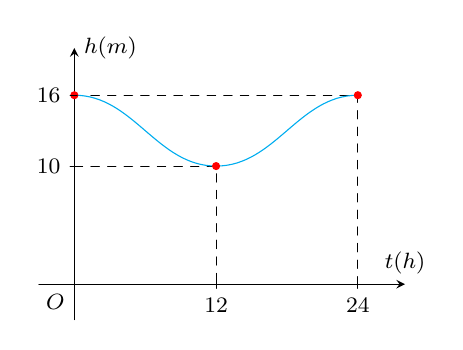
\begin{tikzpicture}[>=stealth,font=\footnotesize,line join=round,line cap=round,x=1.5mm,y=1.5mm]
					 \def\xmin{-3} \def\xmax{28}
					 \def\ymin{-3} \def\ymax{20}
					\draw[->]  (\xmin,0)--(\xmax,0) node [above]{$t (h)$};
					\draw[->] (0,\ymin)--(0,\ymax)  node [right]{$h (m)$};
					\node at (0,0) [below  left]{$O$};
					\draw[dashed] (0,10)-|(12,0) 
						(0,16)-|(24,0); 
					 \draw[cyan]
						(0,16).. controls +(0:5) and +(180:5).. 
						 (12,10).. controls +(0:5) and +(180:5)..
						 (24,16);
					\draw[fill=red,red] (0,16) circle (1.25pt) 
						(12,10) circle (1.25pt) 
						(24,16) circle  (1.25pt);
					\foreach \x in {12,24} 
					\draw(\x,1pt)--(\x,-1.5pt) node [below] {$\x$}; 
					\foreach  \y in {10,16}
					 \draw(1pt,\y)--(-1.5pt,\y) node [left] {$\y$};
				\end{tikzpicture}
		\end{center}
	\end{enumerate}
	 \loigiai{
		\begin{enumerate}
			\item Chiều cao của mực  nước cao nhất là $m+a$ khi $\cos\left(\dfrac{\pi}{12}t\right)=1$ và thấp nhất bằng $m-a$ khi $\cos \left( \dfrac{\pi }{12}t \right)=-1$.\\
			Theo giả thiết, ta  có
			$\heva{&m+a=16\\&m-a=10}  \Leftrightarrow \heva{&m=13\\&a=3.}$
			\item Từ câu a ta có công  thức
			$h=13+3\cos  \left( \dfrac{\pi }{12}t \right)$.\\
			 Do chiều cao của mực nước là $11{,}5$ m nên
			\begin{eqnarray*}
				&&13+3\cos \left( \dfrac{\pi }{12}t  \right) =11{,}5\\
				 &\Leftrightarrow& \cos \left( \dfrac{\pi }{12}t \right) =-\dfrac{1}{2}\\
				&\Leftrightarrow& \hoac{&\dfrac{\pi}{12}t=\dfrac{2\pi}{3}+k2\pi\\&\dfrac{\pi}{12}t=-\dfrac{2\pi}{3}+k2\pi}\left( k\in  \mathbb{Z} \right)\\
				&\Leftrightarrow& \hoac{&t=8+24k\\&t=-8+24k}\left(  k\in \mathbb{Z} \right).
			\end{eqnarray*}
			Ứng với hai thời  điểm trong ngày ta có $t=8$ (giờ) và $t=16$ (giờ).
		\end{enumerate}
	 }
\end{ex}

% nguồn: Ok_TuanLuan_Toan11_Lan2
\begin{ex}%[1D1V5-6]%[ma:28bc2ee0]
	Hội Lim (tỉnh Bắc Ninh) được tổ chức vào mùa xuân thường có trò chơi đánh đu. Khi người chơi đu nhún đều, cây đu sẽ đưa người chơi đu dao động quanh vị trí cân bằng (Hình 39). Nghiên cứu trò chơi này, người ta thấy khoảng cách $h$ (m) từ vị trí người chơi đu đến vị trí cân bằng được biểu diễn qua thời gian $t(s)$ (với $t\geq  0$) bởi hệ thức $h=|d|$ với $d=3\cos\left[\dfrac{\pi}{3}(2t-1)\right]$, trong đó ta quy ước $d>0$ khi vị trí cân bằng ở phía sau lưng người chơi đu và $d<0$ trong trường hợp ngược lại. Vào thời gian $t$ nào thì khoảng cách $h$ là $3$ m; $0$ m?
	\begin{center}
	 \definecolor{darkpastelgreen}{rgb}{0.01, 0.75, 0.24}
	 \definecolor{almond}{rgb}{0.94, 0.87, 0.8}
	\definecolor{arsenic}{rgb}{0.23, 0.27,  0.29}
	 \definecolor{eggplant}{rgb}{0.38, 0.25, 0.32}
	\definecolor{crimson}{rgb}{0.86,  0.08, 0.24}
		\begin{tikzpicture}[line join=round,line cap=round,scale=1,transform shape]
				\clip (-2.5,-2.5) rectangle  (4.5,4.2);
				\tikzset{q_h/.pic={ 
				 \draw[fill=darkpastelgreen] (-.05,4)--(.9,-1.8)
					 ..controls +(30:.05) and +(-30:.05)..(1,-1.75)--(.05,4);
				 \draw[fill=darkpastelgreen] (-.1,4)--(.6,-1.4)
					 ..controls +(30:.05) and +(-30:.05)..(.5,-1.4)--(-.2,4);
				\def\M{ 
					 (-.2,1.76)
					..controls +(-80:.1)  and +(80:.1)..(-.18,1.6)
					..controls  +(-40:.1) and +(30:.06)..(-.18,1.5)--(-.17,1.46)--(-.22,1.44)--(-.19,1.43)--(-.2,1.43)
					..controls  +(-80:.1) and +(-12:.05)..(-.3,1.35)--(-.35,1.28)--(-.55,1.35)
					..controls +(60:.1) and +(-90:.05)..(-.45,1.5) 
					..controls +(100:.1)  and +(140:.05)..(-.38,1.55)
					..controls +(70:.1) and  +(-140:.05)..cycle;
				} 
				\draw\M; 
				 \fill[almond] \M;
				\draw  (-.2,1.76)
					..controls  +(-140:.1) and +(50:.05)..(-.3,1.6)
					(-.2,1.76) 
					..controls +(-120:.1) and  +(40:.05)..(-.25,1.6)
					(-.28,1.578) 
					..controls +(-20:.02)  and +(-150:.02)..(-.22,1.58)
					(-.25,1.568)--(-.23,1.567); 
				\def\A3{ 
					(-.1,.9) 
					 ..controls +(-30:.05) and +(110:0)..(.18,1)
					--(.19,.95) 
					..controls +(-140:.05) and +(30:.05)..(-.1,.7)--cycle; 
				} 
				\fill[arsenic] \A3; 
				 \draw\A3;
				\def\A2{ 
					(-.35,1.28) 
					..controls +(-30:.05) and +(110:.05)..(-.25,1.18) 
					..controls  +(-70:.05) and +(90:.02)..(-.05,.9)
					..controls +(-90:.02)  and +(50:.05)..(-.05,.4)
					..controls  +(-130:.02) and +(50:.05)..(.6,-.8)
					..controls +(-130:.02)  and +(50:.05)..(.9,-1.8)
					..controls +(-130:.2) and +(30:.3)..(-.5,-2.3) 
					..controls +(130:.2) and  +(-90:.1)..(-.2,-1.5)
					..controls +(130:.2) and +(-140:.1)..cycle; 
				 }
				\fill[arsenic] \A2; 
				 \draw\A2;
				 \def\A{
					 (-.55,1.35)
					..controls +(-150:.2)  and +(120:.1)..(-.45,0)
					..controls +(-60:.1) and +(50:.1)..(-.3,-1.6) 
					..controls  +(-10:.1) and +(-120:.1)..(-.15,-1.5)
					..controls +(60:.1) and  +(-120:.1)..(0,-1.45)
					..controls +(120:.3)  and +(-50:.1)..(-.35,.77)
					..controls +(-50:.1) and +(130:.1)..(-.15,.48) 
					..controls +(-50:.1) and +(-130:.1)..(.43,.93) 
					..controls +(-130:.05)  and +(-40:.05)..(.3,1.05)
					..controls +(-130:.05) and  +(40:.05)..(-.05,.75)
					..controls  +(-140:.05) and +(-40:.05)..(-.3,1.15)
					 ..controls +(100:.05) and +(-40:.05)..(-.35,1.28)--cycle;
				} 
				 \fill[eggplant] \A;
				\draw\A; 
				 \def\N{
					 (-.14,1.95)
					..controls +(-80:.1) and  +(80:.1)..(-.17,1.7)
					..controls +(110:.02) and  +(-40:.02)..(-.2,1.76)
					..controls +(-110:.1)  and +(50:.4)..(-.48,1.45)--(-.45,1.35)
					..controls  +(-150:.05) and +(20:.05)..(-.7,1.32)
					..controls  +(50:.05) and +(-120:.05)..(-.65,1.45)
					..controls  +(160:.02) and +(-50:.02)..(-.7,1.48)
					..controls +(160:.02) and +(-50:.02)..(-.8,1.6)--(-.75,1.63) 
					..controls +(-20:.06) and  +(130:.04)..(-.6,1.47)
					..controls +(130:.2)  and +(-90:.1)..(-.7,1.78)
					..controls  +(90:.1) and +(170:.1)..(-.4,1.9)
					..controls  +(20:.1) and +(160:.1)..cycle;
				 }
				\fill[arsenic] \N; 
				\draw\N; 
				 \draw (-.14,1.95)
					 ..controls +(-100:.05) and +(40:.06)..(-.2,1.76)
					 (-.5,1.55)
					..controls +(30:.1) and +(-100:.06)..(-.3,1.76) 
					 (-.6,1.7)
					..controls +(-55:.1) and  +(120:.06)..(-.55,1.5);
				 \def\T1{
					 (.3,1.03)
					..controls  +(60:.05) and +(-120:.05)..(.35,1.15)
					..controls +(60:.05) and  +(-140:.05)..(.45,1.26)
					..controls +(30:.05) and +(60:.04)..(.5,1.22) 
					 ..controls +(30:.03) and +(50:.03)..(.54,1.18)
					..controls +(30:.03)  and +(50:.03)..(.56,1.12)
					..controls +(30:.03) and  +(50:.03)..(.58,1.07)
					 ..controls +(160:.03) and +(40:.03)..(.49,1)
					..controls +(-140:.03) and  +(40:.03)..(.41,.92)--cycle;
				} 
				 \fill[almond] \T1;
				\draw\T1; 
				\fill[crimson](-.27,.4) 
					 ..controls +(-80:.6) and +(-80:.1)..(-.5,-1.9)--(-.45,-1.85)
					..controls +(90:.1) and  +(-80:1)..(-.28,.48)--cycle;
				 \fill[crimson](-.27,.4)
					..controls +(-80:.6) and  +(-80:.1)..(-.2,-1.9)--(-.15,-1.85)
					..controls +(90:.1) and  +(-80:1)..(-.28,.48)--cycle;
					 }}
				\tikzset{no/.pic={ 
				\draw[crimson]  (1.8,-1)
					 ..controls +(150:.4) and +(-120:.5)..(1.7,-1)
					..controls +(30:.4) and +(-40:.3)..(1.75,-1) 
					..controls +(-30:.2)  and +(40:.2)..(1.7,-1.4)
					 (1.75,-1)
					..controls +(-50:.1) and +(20:.1)..(1.7,-1.2); 
					 }}
				\draw(4,-1.25) arc  (-60:-120:6cm);
				\draw[dashed] (4,-1.25)--(1.3,4)--(-2,-1.25) 
					(1.3,4)--(1.3,-2); 
				\node  at (1.5,.5) [rotate=90]{\tiny Vị trí cân bằng};
				 \draw[thick,<->] (.35,-2)--(1.3,-2);
				\node  at (.85,-2) [above]{\tiny $h$};
				\fill (4,-1.25) circle (0.05); 
				 \fill (-2,-1.25) circle (0.05);
				\fill (1.3,4) circle (0.05); 
				 \path
					 (0,0) pic[scale=1,rotate=-20]{q_h}
					(-.88,1.48)  pic[scale=1,scale=.7,rotate=-20]{no};
			\end{tikzpicture}
	\end{center}
	 \loigiai{
		Để khoảng cách $h$ m từ vị trí người chơi đu đến vị trí cân bằng  là $3$ m thì:
		\begin{eqnarray*}
			 &&3\cos\left[\dfrac{\pi}{3}(2t-1)\right]=3\Leftrightarrow\hoac{&3\cos\left[\dfrac{\pi}{3}(2t-1)\right]=3\\&3\cos\left[\dfrac{\pi}{3}(2t-1)\right]=-3}\Leftrightarrow\hoac{&\cos\left[\dfrac{\pi}{3}(2t-1)\right]=1\\&\cos\left[\dfrac{\pi}{3}(2t-1)\right]=-1} \\
			 &\Leftrightarrow&\hoac{&\dfrac{\pi}{3}(2t-1)=k2\pi\\&\dfrac{\pi}{3}(2t-1)=\pi+k2\pi}\Leftrightarrow\hoac{&2t-1=6k\\&2t-1=3+6k}\Leftrightarrow\hoac{&2t=6k+1\\&2t=6k+4}\Leftrightarrow\hoac{&t=3k+\dfrac{1}{2}\\&t=3k+2},(k\in\mathbb{Z}).
		\end{eqnarray*}
		Do $t\geq 0,k\in\mathbb{Z}$ nên $k\in\left\{0;1;2;\ldots\right\}$ khi đó $\hoac{&t\in\left\{\dfrac{1}{2};\dfrac{7}{2};\dfrac{13}{2};\ldots\right\}\\&t\in\left\{2;5;8;\ldots\right\}}\Leftrightarrow t\in\left\{\dfrac{1}{2};2;\dfrac{7}{2};5;\dfrac{13}{2};8;\ldots\right\}$.\\ 
		Vậy $t\in\left(\dfrac{1}{2};2;\dfrac{7}{2};5;\dfrac{13}{2};8;\ldots\right)$ (giây) thì khoảng  cách $h$ là $3$ m.\\
		Để khoảng cách $h$ (m) từ vị trí người chơi đu đến  vị trí cân bằng là $0$ m thì:
		\begin{eqnarray*}
			&&\left|3\cos\left[\dfrac{\pi}{3}(2t-1)\right]\right|=0 
			\Leftrightarrow  3\cos\left[\dfrac{\pi}{3}(2t-1)\right]=0
			\Leftrightarrow  \cos\left[\dfrac{\pi}{3}(2t-1)\right]=0
			\Leftrightarrow\dfrac{\pi}{3}(2t-1)=\dfrac{\pi}{2}+k\pi \\ 
			 &\Leftrightarrow&\dfrac{\pi}{3}(2t-1)
			=\dfrac{\pi}{2}+k\pi\Leftrightarrow 2t-1=\dfrac{3}{2}+3k 
			\Leftrightarrow  2t=\dfrac{5}{2}+3k\Leftrightarrow t=\dfrac{5}{4}+\dfrac{3}{2}k.
		\end{eqnarray*}
	Vậy  $t\in\left\{\dfrac{5}{4};\dfrac{11}{4};\dfrac{17}{4};\ldots\right\}$ (giây) thì khoảng cách $h$ là $0$ m.}
\end{ex}

% nguồn: Ok_TuanLuan_Toan11_Lan2
\begin{ex}%[1D1V5-6]%[ma:98bfc7f4]
	Trong hình minh hoạ dưới đây, khi được kéo ra khơi vị trí cân bằng ở điểm $O$ và buông tay, lực đàn hồi của lò xo khiến vật $A$ gắn ở đầu của lò xo  dao động quanh $O$. Toạ độ $s$ (cm) của $A$ trên trục $Ox$ vào thời điểm $t$ (giây) sau khi buông tay được xác định bởi công thức $s=10\sin\left(10t+\dfrac{\pi}{2}\right)$. Vào các thời điểm nào thì $s=-5\sqrt{3}$ cm?
	\begin{center}
		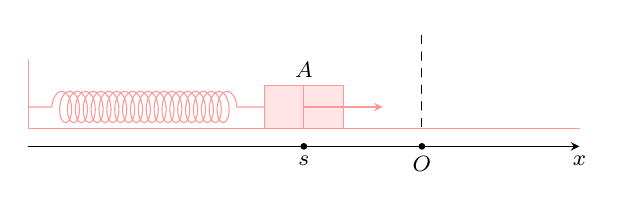
\begin{tikzpicture}[scale=1,font=\footnotesize,line join=round,line cap=round,>=stealth]
				\draw[red!40] (0,.6)--(0,-.27)--(7,-.27); 
				 \draw[red!40,fill=red!10] (3,-0.27) rectangle (3.5,.27)
					(3.5,-0.27) rectangle  (4,.27);
				\draw[red!40,->] (3.5,0)--(4.5,0); 
				 \draw[red!40]
					 [
					decoration={ 
					coil, 
					segment length =  1mm,
					 amplitude = 2mm,
					aspect =  0.5,
					post  length = 3mm,
					pre length =  3mm},
					 decorate] (0,0) -- ++(3,0);
				\draw[,->] (0,-.5) -- (7,-.5) node[below]  {$x$};
				\draw[fill] 
					(3.5,-.5) circle (1pt) node[below]  {$s$}
					(5,-.5) circle  (1pt) node[below] {$O$}
					(3.5,.25) node[above]  {$A$};
				\draw[dashed] (5,-0.25)--(5,1); 
			\end{tikzpicture}
	\end{center}
	\loigiai{ 
		Xét  phương trình
		\begin{eqnarray*}
			&&10\sin\left(10t+\dfrac{\pi}{2}\right)=-5\sqrt{3} 
			\Leftrightarrow \sin\left(10t+\dfrac{\pi}{2}\right)=-\dfrac{\sqrt{3}}{2} \\ 
			&\Leftrightarrow& \sin\left(10t+\dfrac{\pi}{2}\right)=\sin\left(-\dfrac{\pi}{3}\right) 
			 \Leftrightarrow\hoac{&10t+\dfrac{\pi}{2}=-\dfrac{\pi}{3}+k2\pi\\&10t+\dfrac{\pi}{2}=\dfrac{4\pi}{3}+k2\pi},k\in\mathbb{Z}
			\Leftrightarrow\hoac{&t=-\dfrac{\pi}{12}+k\dfrac{\pi}{5}\\&t=\dfrac{\pi}{12}+k\dfrac{\pi}{5}},k\in\mathbb{Z}. 
		\end{eqnarray*}
	Vậy vào  các thời điểm $t=-\dfrac{\pi}{12}+k\dfrac{\pi}{5},\left(k\geq 1,k\in\mathbb{Z}\right)$ và $t=\dfrac{\pi}{12}+k\dfrac{\pi}{5},\left(k\geq 0,k\in\mathbb{Z}\right)$ thì ta thấy được $s=-5\sqrt{3}$ cm.}
\end{ex}

% nguồn: Ok_TuanLuan_Toan11_Lan2
\begin{ex}%[1D1V5-6]%[1D1C5-6]%[ma:e023f5af]
	 Huyết áp là áp lực cần thiết tác động lên thành của động mạch để đưa máu từ tim đến nuôi dưỡng các mô trong cơ thể. Huyết áp được tạo ra do lực co bóp của cơ tim và sức cản của thành động mạch. Mỗi lần tim đập, huyết áp của chúng ta tăng rồi giảm giữa các nhịp. Huyết áp tối đa và huyết áp tối thiểu gọi là huyết áp tâm thu và tâm trương, tương ứng. Chỉ số huyết áp của chúng ta được viết là tâm thu/tâm trương. Chỉ số huyết áp $120/80$ là bình thường. Giả sử một người nào đó có nhịp tim là $70$ lần trên phút và huyết áp của người đó được mô hình hoá bởi hàm số $P(t)=100+20\sin \left( \dfrac{7\pi}{3}t \right)$ ở đó $P(t)$ là huyết áp tính theo đơn vị $\rm\,mmHg$ (milimét thuỷ ngân) và thời gian $t$ tính theo giây.
	\begin{enumerate}
		\item Trong khoảng từ $0$ đến $1$ giây,  hãy xác định số lần huyết áp là $100$ mmHg.
		\item Trong khoảng từ $0$ đến $1$ giây, hãy xác  định số lần huyết áp là $120$ mmHg.
	\end{enumerate}
	 \loigiai{
		\begin{enumerate}
			\item Huyết  áp là $100$ mmHg khi
			\begin{eqnarray*}
				 &&P(t)=100 \\
				&\Leftrightarrow& 100+20\sin  \left( \dfrac{7\pi}{3}t \right)=100\\
				&\Leftrightarrow& \sin \left( \dfrac{7\pi}{3}t \right)=0\\ 
				&\Leftrightarrow& \dfrac{7\pi}{3}t =k\pi\\ 
				&\Leftrightarrow& t=\dfrac{3k}{7} \left(k\in\mathbb{Z}\right). 
			\end{eqnarray*}
			Xét $0<t<1 \Leftrightarrow 0<\dfrac{3k}{7}<1 \Leftrightarrow 0<k<\dfrac{7}{3} \Leftrightarrow k\in \left\{ 1;2 \right\}$ vì  $k\in \mathbb{Z}$.\\
			Vậy trong  khoảng từ $0$ đến $1$ giây, có $2$ lần huyết áp là $100$ mmHg.
			\item Huyết áp là  $120$ mmHg khi
			\begin{eqnarray*}
				 &&P(t)=120 \\
				&\Leftrightarrow& 100+20\sin \left( \dfrac{7\pi}{3}t \right)=120\\ 
				 &\Leftrightarrow& \sin \left( \dfrac{7\pi}{3}t \right)=1\\
				&\Leftrightarrow& \dfrac{7\pi}{3}t=\dfrac{\pi}{2}+k2\pi\\ 
				 &\Leftrightarrow& t=\dfrac{3}{14}+\dfrac{6k}{7} \left(k\in\mathbb{Z}\right).
			\end{eqnarray*}
			Xét $0<t<1 \Leftrightarrow 0<\dfrac{3}{14}+\dfrac{6k}{7}<1  \Leftrightarrow -\dfrac{1}{4}<k<\dfrac{11}{12} \Leftrightarrow k=0$ vì $k\in \mathbb{Z}$.\\
			Vậy trong khoảng từ  $0$ đến $1$ giây, có $1$ lần huyết áp là $120$ mmHg.
		\end{enumerate}
	 }
\end{ex}

% nguồn: Ok_TuanLuan_Toan11_Lan2
\begin{ex}%[1D1V5-6]%[1D1C5-6]%[ma:b2c2eccf]
	Một vệ tinh bay quanh Trái Đất theo một quỹ đạo hình Elip (như hình vẽ): 
	\begin{center}
		\begin{tikzpicture}[scale=0.2,>=stealth,line join=round,line cap=round,font=\footnotesize,transform shape]
				 \definecolor{customblue}{RGB}{2,47,150}
				 \definecolor{customgreen}{RGB}{46,120,23}
				\path (0,0) coordinate (ea); 
				\fill [ball color=customblue] (ea)  circle (7.57);
				\fill [customgreen] (ea)++(-7.57,0).. controls +(.24,-.32) and +(-.61,-.21).. ++(.8,-1.2) 
					..  controls +(.42,.08) and +(-.24,-.05).. ++(1.3,-1)
					..  controls +(.58,-.32).. ++(1,-.58)
					..  controls +(-.16,-.32) and +(-.74,.56).. ++(1,-1.3)
					.. controls +(.05,-.4) and  +(-.08,.53).. ++(1.1,-.69)
					.. controls +(-.34,-.08) and +(-.08,.56)..  +(.88,-1.3)
					.. controls  +(.13,-.56) and +(-.66,.69).. ++(1.67,-2.01)
					.. controls +(.42,-.05)..  ++(.88,-.21)
					.. controls +(.21,0) and +(.4,-.21)..  ++(-.19,.4)
					 .. controls +(-.19,.9).. ++(-.45,1.08)
					.. controls +(-.19,.16) and  +(-.32,0).. ++(.36,.4)
					.. controls +(.11,.03).. ++(0,.24) 
					.. controls +(.26,.32)..  ++(.34,.74)
					.. controls +(-.45,.66).. ++(.5,.79) 
					.. controls +(-.03,1.53) and +(2.12,-.11).. ++(-1.77,2.04) 
					.. controls +(-.37,.74) and +(.21,-.53)..  ++(-1.27,.66)
					.. controls  +(-.42,.24) and +(.05,.37).. ++(-1.16,-.32)
					.. controls +(-.61,-.13) and  +(.26,-.16).. ++(-.45,.37)
					.. controls +(-.37,.05) and +(.45,.63).. ++(-.71,.11) 
					.. controls +(-.77,0) and  +(-.85,.66).. ++(.63,.77)
					.. controls +(.21,-.32) and +(.34,-.32)..  ++(.08,.24)
					.. controls  +(-.08,.24).. ++(.29,.48)
					.. controls +(.03,.95)..  ++(1.06,1.19)
					..  controls +(.26,.03) and +(.29,0).. ++(-.05,.26)
					.. controls +(.21,.29)  and +(-.08,.29).. ++(.29,0)
					.. controls +(.21,.16)  and +(.34,-.13).. ++(.19,.5)
					.. controls +(.11,.34) and  +(.03,-.32).. ++(-.29,.48)
					..  controls +(.05,.24) and +(.05,.24).. ++(-.26,0)
					.. controls +(-.29,-.13) and  +(.21,.42).. ++(-.61,.03)
					.. controls +(-.24,-.16)  and +(.32,.21).. ++(-.29,-.63)
					.. controls +(.16,-.37)  and +(.4,-.45).. ++(-.74,.08)
					..  controls +(.26,.45) and +(-.21,-.48).. ++(1.19,1.48)
					.. controls +(.45,-.29) and +(-.08,.26).. ++(.05,-.5) 
					.. controls +(.34,.03) and +(-.03,-.5)..  ++(.74,.29)
					.. controls +(.29,.19) and  +(.69,-.11).. ++(-.32,.48)
					.. controls  +(-.26,.26) and +(-.61,-.48).. ++(.58,1.06)
					.. controls  +(.4,.08) and +(-.74,-.56).. ++(.24,-.24)
					..  controls +(.74,.19) and +(-1.32,-2.43).. ++(1.19,-.4)
					.. controls +(.71,.19).. ++(1.22,1.08) 
					.. controls +(-.13,.11)..  ++(.24,.29)
					.. controls +(.03,.24)..++(.34,.58) 
					 .. controls +(-.21,.16).. ++(-.37,-.13)
					..  controls +(-.4,.11) and +(1.22,.77).. ++(-2.12,-.79)
					.. controls +(-.56,.24) and +(.45,.24)..  ++(-1.69,.77)
					.. controls +(-.79,-.58) and +(.45,-.03).. ++(-.74,-1.11) 
					.. controls +(-.05,.24) and  +(-.08,.5).. ++(-.32,.42)
					.. controls +(-.03,-.16) and +(.19,-.27).. ($(ea)+(127:7.57)$) arc (127:180:7.57) 
					(ea)++(7.5,.99).. controls +(-.46,.68) and +(.37,-.5)..  ++(-1.39,.55)
					..  controls +(-.32,.56) and +(-.53,.48).. ++(-.05,-.29)
					.. controls +(.63,-.03) and  +(1.71,1.01).. ++(-.42,-1.08)
					.. controls +(-.82,1.75) and +(-1.64,2.06)..  ++(-.19,-.11)
					.. controls +(.85,.16) and +(1.32,1.03).. ++(-.29,-1.24) 
					.. controls  +(-.26,-.5) and +(1.06,.5).. ++(-.63,-1.72)
					..  controls +(.13,-.79) and +(1.24,.13).. ++(-1.64,-1.88)
					..  controls +(.19,.53).. ++(-.4,1.8)
					..  controls +(.19,.53) and +(-.16,-.77).. ++(-.26,1.4)
					.. controls +(-.5,.63)  and +(.85,-.95).. ++(-.34,2.12)
					.. controls  +(.34,.71) and +(1.03,-.03).. ++(-.93,.71)
					..  controls +(-2.06,-.32) and +(.79,-.29).. ++(-1.88,.61)
					.. controls +(-.37,.24) and +(.29,-.42).. ++(0,1.01) 
					.. controls +(1.01,1.51)  and +(-1.83,.03).. ++(2.83,1.48)
					.. controls +(.13,-.42) and  +(-.77,-.42).. ++(1.11,-.37)
					.. controls +(.21,-.34)  and +(-.34,-.16).. ++(1.06,-.24)
					 .. controls +(.42,.42) and +(.4,.21).. ++(-.21,.37)
					 .. controls +(-.29,-.08) and +(-.08,-.26).. ++(-.45,.4)
					.. controls +(-.21,.32) and +(.05,-.61)..  ++(-.45,.08)
					.. controls +(-.98,1.08) and +(-.48,.21)..  ++(-.32,.08)
					.. controls +(.19,-.16) and +(.29,.13)..  ++(-.4,-.4)--++(-.09,.13)
					 .. controls +(.26,.16) and +(.16,-.08).. ++(-.21,.69)
					..  controls +(-.19,-.08) and +(.32,.26).. ++(-.63,-.19)
					.. controls +(-.29,-.11) and +(1.14,-.37)..  ++(-1.35,-.32)
					.. controls +(.11,.53) and +(-.34,.11).. ++(.61,.56) 
					.. controls +(-.03,.13)  and +(.32,-.24).. ++(.03,.4)
					.. controls +(.66,.13).. ++(.74,.45) 
					.. controls +(.4,.05).. ++(.4,.45) 
					.. controls +(.24,-.29) and +(-.11,-.69)..  ++(.98,.03)
					.. controls +(.56,.24)  and +(-.34,-.45).. ($(ea)+(69:7.57)$) arc (69:8:7.57)
					 (ea)++(5.37,-2.67)
					.. controls +(-.26,-1.08) and +(-.37,-1.14)..  ++(.4,-.29)
					.. controls +(.32,.69) and +(.45,.63).. ++(-.4,.29) 
					(ea)++(1.6,6.9).. controls  +(.98,.21) and +(.13,.19).. ++(.69,-.26)
					.. controls  +(-.66,.03) and +(-.32,-.37).. ++(-.69,.26);
				\path 
					 (ea)++(0:2) coordinate (O)
					($({11*cos  (65)},{8.5*sin (65)})+(O)$) coordinate (V)
					 (ea)++(50:7.57) coordinate (V1)
					($({11*cos (-80)},{8.5*sin (-80)})+(O)$)  coordinate (V2)
					(ea)++(-65:7.57) coordinate (V3); 
				\draw (O) ellipse (11  and 8.5);
				\draw  [<->] (7.57,0)--(13,0) node [below,midway] {\scalebox{4}{1\,000}};
				\draw [<-] (-9,0)--++(180:2) node [pos=1,left]  {\scalebox{4}{$h=100$}};
				\draw  [<-] (-7.57,0)--++(0:2);
				\draw [<->] (V)--(V1) node [midway,below right] {\scalebox{4}{$h$}}; 
				\draw [<->] (V2)--(V3) node [midway,above=25pt,sloped] {\scalebox{4}{$250$}}; 
				\draw [fill=white] (V) circle (4pt) node [above right]  {\scalebox{4}{Vệ tinh}};
			\end{tikzpicture}
	\end{center}
	Độ cao $h$ (tính bằng kilômet) của vệ tinh so với bề  mặt Trái Đất được xác định bởi công thức $h=550+450\cdot\cos\dfrac{\pi}{50}t$. Trong đó $t$ là thời gian tính bằng phút kể từ lúc vệ tinh bay vào quỹ đạo. Người ta cần thực hiện một thí nghiệm khoa học khi vệ tinh cách mặt đất $250$ km. Trong khoảng $60$ phút đầu tiên kể từ lúc vệ tinh bay vào quỹ đạo, hãy tìm thời điểm để có thể thực hiện thí nghiệm đó?
	\loigiai{ 
		Ta có 
		\begin{align*}
			550+450\cdot\cos\dfrac{\pi}{50}t=250 &\Leftrightarrow \cos\dfrac{\pi}{50}t=-\dfrac{2}{3}.\\ 
			\text{(bấm máy) }\hoac{&\dfrac{\pi}{50}t\approx 2{,}3+k2\pi\\&\dfrac{\pi}{50}t\approx -2{,}3+k2\pi} 
			&\Leftrightarrow 
			\hoac{&t\approx  36{,}61+k100\\&t\approx -36{,}61+k100},k\in \mathbb{Z}.
		\end{align*}
		Vậy trong khoảng $60$ phút  đầu tiên kể từ lúc vệ tinh bay vào quỹ đạo, tại thời điểm $t\approx 36{,}61$ (phút) thì ta có thể thực hiện thí nghiệm đó.
	} 
\end{ex}

% nguồn: Ok_TuanLuan_Toan11_Lan2
\begin{ex}%[1D1V5-6]%[1D1C5-6]%[ma:2201479d]
	Trong môn cầu lông, khi phát cầu, người chơi cần đánh cầu qua khỏi lưới sang phía sân đối phương và không được để cho cầu rơi ngoài biên. Trong mặt phẳng toạ độ $Oxy$, chọn điểm có tọa độ $\left( O;y_0 \right)$ là điểm xuất phát thì phương trình quỹ đạo của cầu lông khi rời khỏi mặt vợt là 
	$y=\dfrac{-g\cdot x^2}{2\cdot v_0^2\cdot  \cos^2\alpha} +\tan\alpha\cdot x+y_0$; trong đó:
	\begin{itemize} \allowdisplaybreaks
		\item $g$ là gia tốc  trọng trường (thường được chọn là $9{,}8\rm\,m/s^2$);
		\item $\alpha$ là góc phát cầu  (so với phương ngang của mặt đất);
		 \item $v_0$ là vận tốc ban đầu của cầu;
		\item $y_0$ là khoảng cách từ vị  trí phát cầu đến mặt đất.
	\end{itemize}
	Đây là một hàm số bậc hai nên quỹ đạo  chuyển động của cầu lông là một parabol.\\
	Một người chơi cầu lông phát quả cầu. Vị trí cầu rơi chạm đất cách vị trí người chơi $6{,}68$ m (tầm bay xa). Quan sát hình bên dưới, hỏi người chơi đã phát cầu góc khoảng bao nhiêu độ so với mặt đất? ( biết cầu  rời mặt vợt ở độ cao $0{,}7$ m so với mặt đất và vận tốc xuất phát của cầu là $8$ m/s, bỏ qua sức cản của gió và xem quỹ đạo của cầu luôn nằm trong mặt phẳng phẳng đứng). \\ [.2cm]
	\centerline{ 
	\begin{tikzpicture}[scale=0.5,>=stealth,line join=round,line cap=round,font=\footnotesize]
			 \def\xmin{-1}
			 \def\xmax{14}
			\def\ymin{-1} 
			 \def\ymax{5}
			\def\f{-.075*(\x)^2+.55*(\x)+2} 
			\draw  [smooth,samples=100] plot [domain=0:10] (\x,{\f});
			\draw [->] (\xmin,0)--(\xmax,0) node [below,xshift=-3pt]  {$x$};
			\draw [->] (0,\ymin)--(0,\ymax) node  [left,yshift=-4pt] {$y$};
			 \draw [->] (0,2)--++(30:2);
			\draw [dashed]  (0,2)--++(0:2);
			\draw  (.5,2) arc (0:30:.5)
				(1,2.2) node  {$\alpha$};
			\draw [fill] (0,0)  circle (1pt) node [below left] {$O$}
				(0,2) circle (1pt) node [left] {$0{,}7$  m}
				(4,3) circle  (1pt)
				(10,0) circle (1pt) node [below] {Điểm chạm đất} 
				(4,1) node  {$y=\dfrac{-gx^2}{2v_0^2\cos^2\alpha}+\tan\alpha+y_0$};
		\end{tikzpicture}
	} 
	\loigiai{ 
		Với $g=9{,}8$ $\rm  m/s^2$, vận tốc ban đầu $v_0=8$ $\rm m/s$ thì phương trình quỹ đạo của cầu là\\
		$y=\dfrac{-g\cdot  x^2}{2\cdot v_0^2\cdot \cos^2\alpha}+\tan\alpha \cdot x+y_0$.\\
		Khoảng cách từ vị trí người này đến vị trí cầu rơi chạm đất (tầm bay xa) là $6{,}68$ m nghĩa là $x=6{,}68$ m.\\ 
		 Ta có
		\begin{align*}
			&\dfrac{-9{,}8\cdot (6{,}68)^2}{128\cdot \cos^2\alpha  }+\tan\alpha\cdot 6{,}68+0,7=0\\
			\Leftrightarrow& \dfrac{-9,8\cdot (6{,}68)^2}{128}\left( 1+\tan^2\alpha \right)+\tan\alpha\cdot 6{,}68+0,7=0\\ 
			\Leftrightarrow& 
			\hoac{&\tan\alpha \approx  1{,}378\\&\tan\alpha \approx 0{,}576} \Leftrightarrow
			\hoac{&\alpha  \approx 54{,}04^\circ\\&\alpha \approx 29{,}97^\circ.}
		\end{align*}
		Vậy người chơi đã phát cầu một góc gần $54^\circ $ hoặc gần  $30^\circ $ so với mặt đất.
	 }
\end{ex}

% nguồn: Ok_TuanLuan_Toan11_Lan2
\begin{ex}%[1D1V5-6]%[ma:62485fce]
	\immini{ 
	Chiều cao $h$ (m) của một cabintrên vòng quay vào thời điểm $t$ (s) giây sau khi bắt đầu chuyển động được cho bởi công thức $h(t)=30+20\sin\left( \dfrac{\pi}{25}t+\dfrac{\pi}{3}  \right)$.
	\begin{enumerate}
		\item Cabin đạt độ cao tối đa là bao  nhiêu?
		\item Sau bao nhiêu giây thì cabin đạt độ  cao $40\rm\, m$ lần đầu tiên?
	\end{enumerate}
	}{ 
	\begin{tikzpicture}[>=stealth,line join=round,line cap=round,font=\footnotesize,scale=.8,declare function={d=0.32; R=2.2; r=1.21;}]
			\tikzset{ 
				 thungdu/.pic={
			\draw[fill=cyan!15,teal,ultra thick,preaction={fill=white}]  (d,d/2) arc (0:-180:d and d);
			} 
			} 
			\draw  (0,0) circle (.95*R);
			 \draw[line width=3pt] (0,0) circle (R) circle (r);
			\foreach \i  in {0,...,11}{
				\begin{scope}[rotate=30*\i]
				 \clip (-3:R)--(0,0)--(3:R);
				\draw  (-3:R)--(0,0)--(3:R);
				\foreach \i  in {1,...,11}
				\draw ($(0,0)!\i/12!(-3:R)$)--++(120:2); 
				\end{scope}
			 }
			 \foreach \i in {1,...,12}
			\path ({-90+30*\i}:R) pic{thungdu}; 
			\draw[fill]  (-1.4,-3.6) rectangle (1.4,-3.4);
			\draw[fill]  (-1.1,-3.4) rectangle (1.1,-3.2);
			\draw[line  width=3pt] (-.65,-3.4)--(0,0)--(.65,-3.4);
			 \draw[fill] (0,0) circle (8pt);
			\draw [<->] (0,0)++(-30:R)++(0:.5)--++(-90:2.5) node  [midway,right] {$h (t)$};
		\end{tikzpicture}
	} 
	 \loigiai{
		\begin{enumerate}
			\item 
			Ta có $-1\le\sin\left( \dfrac{\pi}{25}t+\dfrac{\pi}{3}  \right)\le1 \Rightarrow -20\le20\sin\left(\dfrac{\pi}{25}t+\dfrac{\pi}{3}\right)\le20$.\\
			Do đó $10\le h(t)\le50$.\\ 
			 Vậy độ cao lớn nhất của mỗi cabin là $50$ (m).
			 \item
			Cabin ở độ cao $40$ (m) ở lần đầu tiên, giải phương  trình
			\begin{eqnarray*}
				 &&30+20\sin\left(\dfrac{\pi}{25}t+\dfrac{\pi}{3}\right)=40\\
				&\Leftrightarrow&  \sin\left(\dfrac{\pi}{25}t+\dfrac{\pi}{3}\right)=\dfrac{1}{2}\\
				 &\Leftrightarrow&
				\hoac{&\dfrac{\pi}{25}t+\dfrac{\pi}{3}=\dfrac{\pi}{6}+k2\pi\\ &\dfrac{\pi}{25}t+\dfrac{\pi}{3}=\pi-\dfrac{\pi}{6}+k2\pi}, \quad (k\in \mathbb{Z})  \\
				 &\Leftrightarrow&
				\hoac{&t=-\dfrac{25}{6}+50k \\  &t=\dfrac{25}{2}+50k}\\
			\end{eqnarray*}
			Khi  cabin đạt độ cao $40$ m lần đầu tiên thì $t$ nhận giá trị không âm và nhỏ nhất. \\
			Do  đó $t=\dfrac{25}{2}$ (giây).
		\end{enumerate}
	 }
\end{ex}

% nguồn: Ok_TuanLuan_Toan11_Lan2
\begin{ex}%[1D1V5-6]%[1D1C5-6]%[ma:6be81778]
	Vận tốc $v_1$ (cm/s) của con  lắc đơn thứ nhất và vận tốc $v_2$ (cm/s) của con lắc đơn thứ hai theo thời gian $t$ (giây) được cho bởi các công thức:
	$v_1(t)=-4\cos\left(\dfrac{2t}{3}+\dfrac{\pi}{4}\right)$ và $v_2(t)=2\sin\left(2t+\dfrac{\pi}{6}\right)$. 
	Xác định các thời  điểm $t$ mà tại đó
	\begin{enumerate}
		\item Vận tốc của con lắc đơn thứ nhất bằng  $2$ cm/s;
		\item Vận tốc của con lắc  đơn thứ nhất gấp hai lần vận tốc của con lắc đơn thứ hai.
	\end{enumerate}
	\loigiai{ 
		\begin{enumerate} \allowdisplaybreaks
			\item Vì vận tốc của con lắc đơn  thứ nhất bằng $2$ cm/s nên $v_1(t)=2$.
			\begin{align*}
				 &-4\cos\left(\dfrac{2t}{3}+\dfrac{\pi}{4}\right)=2\\
				&\Leftrightarrow\cos\left(\dfrac{2t}{3}+\dfrac{\pi}{4}\right)=-\dfrac{1}{2}\\ 
				&\Leftrightarrow\hoac{&\dfrac{2t}{3}+\dfrac{\pi}{4}=\dfrac{2\pi}{3}+k2\pi\\  &\dfrac{2t}{3}+\dfrac{\pi}{4}=\dfrac{4\pi}{3}+k2\pi}\\
				&\Leftrightarrow\hoac{&\dfrac{2t}{3}=\dfrac{5\pi}{12}+k2\pi\\  &\dfrac{2t}{3}=\dfrac{13\pi}{12}+k2\pi}\\
				 &\Leftrightarrow\hoac{&t=\dfrac{5\pi}{8}+k3\pi\\ &t=\dfrac{13\pi}{8}+k3\pi}, (k\in\mathbb{Z}^+)
			\end{align*}
			Vậy vận tốc con lắc thứ nhất bằng $2$ cm/s  vào các thời điểm $t=\dfrac{5\pi}{8}+k3\pi, k\in \mathbb{Z}^+$ và $t=\dfrac{13\pi}{8}+k3\pi, k\in \mathbb{Z}^+$.
			\item Vì vận tốc con lắc đơn thứ nhất gấp đôi vận  tốc của con lắc đơn thứ hai nên $v_1(t)=2v_2(t)$.
			\begin{align*}
				&-4\cos\left(\dfrac{2t}{3}+\dfrac{\pi}{4}\right) =2\cdot2\sin\left(2t+\dfrac{\pi}{6}\right)\\ 
				&\Leftrightarrow  \cos\left(\dfrac{2t}{3}+\dfrac{\pi}{4}\right) =-\sin\left(2t+\dfrac{\pi}{6}\right)\\
				 &\Leftrightarrow \cos\left(\dfrac{2t}{3}+\dfrac{\pi}{4}\right) =\sin\left(-2t-\dfrac{\pi}{6}\right)\\
				 &\Leftrightarrow \cos\left(\dfrac{2t}{3}+\dfrac{\pi}{4}\right) =\cos\left(2t+\dfrac{2\pi}{3}\right)\\
				&\Leftrightarrow \hoac{&2t+\dfrac{2\pi}{3}=\dfrac{2t}{3}+\dfrac{\pi}{4}+k2\pi\\  &2t+\dfrac{2\pi}{3}=-\dfrac{2t}{3}-\dfrac{\pi}{4}+k2\pi}\\
				&\Leftrightarrow  \hoac{&\dfrac{4t}{3}=-\dfrac{5\pi}{12}+k2\pi\\ &\dfrac{8t}{3}=-\dfrac{11\pi}{12}+k2\pi}\\
				&\Leftrightarrow \hoac{&t=-\dfrac{5\pi}{16}+k\dfrac{3\pi}{2}\\ &t=-\dfrac{11\pi}{32}+k\dfrac{3\pi}{4}},  (k\in\mathbb{Z}^+)\\
				&\Leftrightarrow \hoac{&t=\dfrac{19\pi}{16}+l\dfrac{3\pi}{2}\\ &t=\dfrac{13\pi}{32}+l\dfrac{3\pi}{4}},  (l\in\mathbb{Z}^+; l=k+1).
			\end{align*}
			Vậy vào các thời điểm $t=\dfrac{19\pi}{16}+l\dfrac{3\pi}{2},  l\in \mathbb{Z}^+$ và $t=\dfrac{13\pi}{32}+l\dfrac{3\pi}{4}, l\in \mathbb{Z}^+$ thì vận tốc con lắc đơn thứ nhất gấp đôi vận tốc con lắc đơn thứ hai.
		\end{enumerate}
	 }
\end{ex}

% nguồn: Ok_TuanLuan_Toan11_Lan2
\begin{ex}%[1D1V5-6]%[1D1C5-6]%[ma:9ec19cc4]
	Một cây cầu có dạng cung $OA$ của đồ thị hàm số $y=4{,}8\sin\dfrac{x}{9}$ và được mô tả trong hệ trục  tọa độ với đơn vị trục là mét như ở hình dưới đây:
	\begin{center}
		\begin{tikzpicture}[scale=1,>=stealth,font=\footnotesize,line join=round,line cap=round,x=4mm,y=5mm]
				\def\xmin{-1.5} \def\xmax{30}  \def\ymin{-1.5} \def\ymax{6}
				\draw[->] (\xmin,0)--(\xmax,0) node  [below]{$x$};
				\draw[->] (0,\ymin)--(0,\ymax)  node [right]{$y$};
				\node at (0,0)  [below left]{$O$};
				 \node at (9*pi,0) [below]{$A$};
				\clip (\xmin+0.1,\ymin+0.1) rectangle (\xmax-0.1,\ymax-0.1); 
				 \draw[smooth,samples=400,domain=0:28.3] plot (\x,{4.8*sin (\x/9 r)});
				\draw[fill,black] (0,0) circle  (1pt)
					 (9*pi,0) circle (1pt);
			\end{tikzpicture}
	\end{center}
	\begin{enumerate}
		\item Giả sử chiều rộng của con sông là độ dài đoạn thẳng  $OA$. Tìm chiều rộng đó (Làm tròn kết quả đến hàng phần mười).
		\item Một sà lan chở khối hàng hóa được xếp thành hình hộp chữ nhật với độ cao $3{,}6$ m so với  mực nước sông sao cho sà lan có thể đi qua được gầm cầu. Chứng minh rằng chiều rộng của khối hàng hóa đó phải nhỏ hơn $13{,}1$ m.
		\item Một sà lan khác cũng chở khối hàng hóa được xếp thành hình hộp chữ nhật với chiều rộng của khối hàng hóa đó là $9$ m sao cho sà lan có thể đi qua được gầm cầu. Chứng minh rằng chiều cao của khối hàng hóa đó phải nhỏ hơn $4{,}3$ m. 
	\end{enumerate}
	 \loigiai{\allowdisplaybreaks
		\begin{enumerate}
			\item Giải  phương trình
			\begin{align*}
				y=0 \Leftrightarrow  4{,}8\sin\dfrac{x}{9}=0 \Leftrightarrow \sin\dfrac{x}{9}=0 \Leftrightarrow \dfrac{x}{9}=k\pi \Leftrightarrow x=k9\pi \left( k\in \mathbb{Z} \right).
			\end{align*}
			 Do đó đồ thị cắt trục $Ox$ tại các điểm có hoành độ $0;9\pi; 18\pi; \ldots$.\\
			Vì  thế $A(9\pi;0)$ nên chiều rộng của con sông là $OA=9\pi \approx 28{,}3$ m.
			\item Xét đường  thẳng $y=3{,}6$.\\
			Ta có $y=4{,}8\sin\dfrac{x}{9} \le 4{,}8$ nên đường thẳng $y=3{,}6$ cắt một phần đồ thị của hàm số $y=4{,}8\sin\dfrac{x}{9}$ tại hai  điểm $M\left(x_1;3{,}6\right)$, $N\left(x_2;3{,}6\right)$.\\
			Giải phương trình $4{,}8\sin\dfrac{x}{9}=3{,}6 \Leftrightarrow \sin\dfrac{x}{9} =\dfrac{3}{4}\  (1)$. \\
			 Gọi $x_1$, $x_2$ là hai nghiệm dương nhỏ nhất của $(1)$.\\
			Vì $-1\le \dfrac{3}{4}\le 1$ nên tồn tại một số $\alpha \in \left[-\dfrac{\pi}{2};\dfrac{\pi}{2}\right]$ sao cho $\sin\alpha=\dfrac{3}{4}$.\\ 
			 Ta có $\sin\dfrac{x}{9}=\sin\alpha \Leftrightarrow $
			 $\hoac{&\dfrac{x}{9}=\alpha+k2\pi\\&\dfrac{x}{9}=\pi-\alpha+k2\pi} \Leftrightarrow \hoac{&x=9\alpha+k18\pi\\&x=9\pi-9\alpha+k18\pi.}$\\
			 Do $x_1; x_2\in (0;9\pi)$ nên $x_1 \approx 9\alpha \approx 7{,}6325$; $x_1 \approx 9\pi-9\alpha \approx 20{,}6418$ nên $x_2-x_1<13{,}1$.\\
			Vậy chiều  rộng của khối hàng hoá bé hơn $13{,}1$ m.
			\item Cho $0<m<4{,}8$ đường thẳng $y=m$ cắt $(C)$ tại hai điểm $P\left(x_3;m\right)$, $Q\left(x_4;m\right)$, với $x_3$, $x_4$ là hai nghiệm dương nhỏ nhất của phương trình $4{,}8\sin\dfrac{x}{9}=m$ $(2)$ và thỏa mãn  $x_4-x_3=9$.\\
			$(2) \Leftrightarrow \sin\dfrac{x}{9}=\dfrac{m}{4{,}8}$. \\ 
			Vì  $0<\dfrac{m}{4{,}8}<1$ nên $\exists \beta \in \left[-\dfrac{\pi}{2};\dfrac{\pi}{2} \right]$ sao cho $\sin\beta=\dfrac{m}{4{,}8}$ $(*)$.\\
			 Khi đó $(2)$ trở thành $\sin\dfrac{x}{9}=\sin\beta$
			$ \Leftrightarrow  \hoac{&x=9\beta+k18\pi\\&x=9(\pi-\beta)+k18\pi}, \quad k\in \mathbb{Z}.$\\
			Hai nghiệm dương  nhỏ nhất của $(2)$ là $x_3=9\beta$, $x_4=9(\pi-\beta)$.\\
			Ta có  $x_4-x_3=9(\pi-\beta)-9\beta=0$.\\
			 Do vậy $m=4{,}8\sin\beta$ hay $m=4{,}8\sin\dfrac{\pi-1}{2} \approx 4{,}2124<4{,}3$.\\
			Vậy chiều cao của mỗi khối  hàng hoá bé hơn $4{,}3$ m.
		\end{enumerate}
	} 
\end{ex}

% nguồn: Ok_TuanLuan_Toan11_Lan2
\begin{ex}%[1D1V5-6]%[1D1C5-6]%[ma:780040d4]
	Một chất điểm chuyển động đều theo chiều ngược chiều kim đồng hồ trên đường tròn bán kính $5$ cm. Khoảng cách $h$ cm từ chất điểm đến trục hoành được tính theo  công thức $h=\big|y\big|$, trong đó $y=a\sin\left( \dfrac{\pi}{5}t \right)$ với $t$ là thời gian chuyển động của chất điểm tính bằng giây $( t\ge 0)$ và chất điểm bắt đầu chuyển động từ vị trí $A$.
	\begin{enumerate}
		\item Chất điểm chuyển động một vòng hết bao nhiêu  giây?
		\item Tìm giá trị của  $a$.
		\item Tìm thời điểm sao cho chất điểm ở vị trí có $h=2{,}5$ cm và nằm  phía dưới trục hoành trong một vòng quay đầu tiên.
		\begin{center}
			\begin{tikzpicture}[scale=1,>=stealth,font=\footnotesize,line join=round,line cap=round,x=3mm,y=3mm]
					\def\xmin{-7} \def\xmax{7} 
					\def\ymin{-7} \def\ymax{7} 
					\draw[->] (\xmin,0)--(\xmax,0) node [below]{$x$}; 
					\draw[->] (0,\ymin)--(0,\ymax) node  [left]{$y$};
					\node at  (0,0) [below left]{$O$};
					\path (0,0)  coordinate (O)
						 (0:5) coordinate (A)
						 (45:5) coordinate (B)
						 ($(O)!(B)!(A)$) coordinate (H);
					\draw[cyan] (0,0)  circle (5);
					\draw[dashed]  (O)--(B) node[midway,above]{$5$}--(H) node[midway,left]{$h$};
					\draw[black,fill] (O) circle  (1.25pt)
						 (A) circle (1.25pt)
						(B)  circle (1.25pt)
						(H) circle (1.25pt); 
					\path  (B) node[above right]{$A$};
				\end{tikzpicture}
		\end{center}
	\end{enumerate}
	\loigiai{ 
		\begin{enumerate}
			\item Xét $h=0$ hay  $a\sin\left( \dfrac{\pi}{5}t \right)=0 \Leftrightarrow t=5k$ với $k\in \mathbb{Z}$ và $k\ge 0$.\\
			Ta nhận thấy, từ thời điểm ban đầu, cứ sau $5$ giây, khoảng cách từ chất điểm đến trục  hoành lại bằng $0$.\\
			Suy ra sau mỗi $5$ giây, chất điểm chuyển động được nửa vòng.\\ 
			Vậy chất điểm chuyển động một vòng hết 10 giây. 
			\item Do chất điểm chuyển động một vòng hết $10$ giây nên khi $t=2{,}5$ giây thì chất điểm chuyển động được  một phần tư vòng theo chiều dương, suy ra tại $t=2{,}5$ ta có \\
			\centerline{$y=\big|y\big|=h=5 \Leftrightarrow a\sin\left(\dfrac{\pi}{5}\cdot\dfrac{5}{2}\right) =5  \Leftrightarrow a=5$.
			} 
			\item Khi chất điểm nằm phía dưới trục hoành và có vị trí $h=2{,}5$ cm  ta có
			\begin{eqnarray*}
				&&y=-2{,5} \\ 
				&\Leftrightarrow& 5\sin\left(\dfrac{\pi}{5}t\right)=2{,5}  \\
				&\Leftrightarrow&  \sin\left(\dfrac{\pi}{5}t\right)=\dfrac{1}{2} \\
				&\Leftrightarrow&  \sin\left(\dfrac{\pi}{5}t\right)=\sin\dfrac{\pi}{6} \\
				&\Leftrightarrow& \hoac{&\dfrac{\pi}{5}t=\dfrac{\pi}{6}+k2\pi \\ &\dfrac{\pi}{5}t=\dfrac{5\pi}{6}+k2\pi}, \quad k\in  \mathbb{Z} \\
				 &\Leftrightarrow& \hoac{&t=\dfrac{5}{6}+10k \\ &t=\dfrac{25}{6}+10k.}
			\end{eqnarray*}
			Vì là thời điểm đầu tiên nên $t$ nhận giá trị không âm và  nhỏ nhất. \\
			Do đó $t=\dfrac{5}{6}$.  \\
			Vậy thời điểm  đầu tiên chất điểm ở vị trí $h=2{,}5$ và phía dưới trục hoành là $\dfrac{5}{6}$ (giây).
		\end{enumerate}
	} 
\end{ex}

% nguồn: Ok_TuanLuan_Toan11_Lan2
\begin{ex}%[1D1V5-6]%[ma:fdc15bf4]
	Một quả bóng được ném xiên một góc $\alpha$ $\left( 0^\circ \le \alpha \le 90^\circ \right)$  từ mặt đất với tốc độ $v_0$ $\rm\left(m/s\right)$. Khoảng cách theo phương ngang từ vị trí ban đầu của quả bóng đến vị trí bóng chạm đất được tính bởi công thức $d=\dfrac{v_0^2\sin2\alpha}{10}$.
	\begin{enumerate}
		\item Tính khoảng cách $d$ khi bóng được ném đi với tốc độ ban đầu $10$ $\rm m/s$ và góc ném là $30^\circ$  so với phương ngang.
		\item Nếu tốc độ ban đầu của bóng là $10$ $\rm m/s$ thì cần  ném bóng với góc bao nhiêu độ để khoảng cách $d$ là $5$ $\rm m$?
	\end{enumerate}
	\loigiai{ 
		\begin{enumerate}
			\item 
			Ta có vận tốc ban  đầu $v_0=10$ $\rm(m/s)$, góc ném $\alpha=30^\circ$ so với phương ngang.\\
			Áp dụng  công thức $d=\dfrac{v_0^2\sin2\alpha}{10}$ ta được
			\begin{align*}
				d=\dfrac{10^2\cdot\sin60^\circ}{10} =5\sqrt{3} \approx  8{,}66\ \rm (m).
			\end{align*}
			 \item
			Với  khoảng cách $d$ là $5$ (m), áp dụng công thức $d=\dfrac{v_0^2\sin2\alpha}{10}$ ta có
			\begin{eqnarray*}
				&&d=5 \\ 
				&\Leftrightarrow& \dfrac{10^2\cdot\sin2\alpha}{10} =5  \\
				&\Leftrightarrow&  10\sin2\alpha=5\\
				&\Leftrightarrow&  \sin2\alpha=\dfrac{1}{2}\\
				&\Leftrightarrow& \hoac{&2\alpha=30^\circ+k360^\circ\\  &2\alpha=150^\circ+k360^\circ} \\
				&\Leftrightarrow&  \hoac{&\alpha=15^\circ+k180^\circ\\ &\alpha=75^\circ+k180^\circ.}
			\end{eqnarray*}
			Vì $0^\circ \le \alpha \le 90^\circ$ nên $\alpha=15^\circ$ hoặc $\alpha=75^\circ$. \\ 
			Vậy chọn góc ném $\alpha=15^\circ$ hoặc $\alpha=75^\circ$. 
		\end{enumerate}
	} 
\end{ex}

% nguồn: Ok_TuanLuan_Toan11_Lan2
\begin{ex}%[1D1V5-6]%[1D1C5-6]%[ma:ad82b2a7]
	Hằng ngày, mực nước của một con kênh lên xuống theo thủy triều. Độ sâu $h$ (m) của mực nước trong kênh tính theo thời gian $t$ (giờ) trong một ngày $(0\le t<24)$ cho bởi  công thức $h=3\cos \left( \dfrac{\pi t}{6}+1 \right)+12$. Tìm $t$ để độ sâu của mực nước là
	\begin{enumEX}{3}
		\item  $15$ m.
		\item  $9$ m.
		\item  $10{,}5$ m.
	\end{enumEX}
	\loigiai{ 
		\begin{enumerate}
			\item Độ sâu  của mực nước là $15$ m thì $h = 15$.\\
			 Khi đó
			\begin{eqnarray*}
				&& 15=3\cos \left(  \dfrac{\pi t}{6}+1 \right)+12 \\
				&\Leftrightarrow& \cos \left( \dfrac{\pi t}{6}+1 \right)=1  \\
				&\Leftrightarrow& \cos \left( \dfrac{\pi t}{6}+1 \right) =\cos  0 \\
				&\Leftrightarrow& \dfrac{\pi t}{6}+1 =k2\pi \\ 
				&\Leftrightarrow&  t=\dfrac{6\left( k2\pi -1 \right)}{\pi}; k\in \mathbb{Z}.
			\end{eqnarray*}
			Vì $0  < t \le 24$ nên
			\begin{eqnarray*}
				&&0 < \dfrac{6(k2\pi-1)}{\pi } \le 24 \\ 
				&\Leftrightarrow& 0 < k2\pi-1 \le 4\pi \\ &\Leftrightarrow&  \dfrac{1}{2\pi} < k \le \dfrac{4\pi-1}{2\pi}.
			\end{eqnarray*}
			Suy  ra $ 0<k\le 2$.\\
			Lại  do $k\in \mathbb{Z} \Rightarrow k\in \{1;2\} \Rightarrow t\in \left\{ \dfrac{6\left(2\pi-1\right)}{\pi}; \dfrac{6\left(4\pi-1\right)}{\pi} \right\}$.
			\item Độ sâu của mực nước là $9$ m  thì $h=9$.\\
			Khi  đó
			\begin{eqnarray*}
				&&9=3\cos\left(\dfrac{\pi t}{6}+1\right)+12  \\
				&\Leftrightarrow& \cos\left(\dfrac{\pi t}{6}+1\right)  =-1 \\
				&\Leftrightarrow& \cos \left(\dfrac{\pi t}{6}+1\right)  =\cos\pi \\
				&\Leftrightarrow& \dfrac{\pi t}{6}+1=\pi +k2\pi \\ &\Leftrightarrow& t=\dfrac{6\left( k2\pi  +\pi -1 \right)}{\pi} \quad \left( k\in \mathbb{Z} \right)
			\end{eqnarray*}
			Vì  $0\le t<24$ nên $0\le \dfrac{6(k2\pi +\pi -1)}{\pi}\le 24 \Leftrightarrow 0<k\le 1$.\\
			Lại do $k\in \mathbb{Z}\Rightarrow k=1\Rightarrow t=\dfrac{6\left( 3\pi  -1 \right)}{\pi }$.
			\item Độ  sâu của mực nước là $10{,}5$ m thì $h=10,5$.\\
			 Khi đó
			\begin{eqnarray*}
				&&10,5=3\cos \left( \dfrac{\pi  t}{6}+1 \right)+12 \\
				&\Leftrightarrow& \cos \left(  \dfrac{\pi t}{6}+1 \right) =-\dfrac{1}{2} \\
				&\Leftrightarrow& \cos \left( \dfrac{\pi t}{6}+1 \right)=\cos \dfrac{2\pi  }{3} \\
				 &\Leftrightarrow&
				\hoac{&\dfrac{\pi t}{6}+1=\dfrac{2\pi}{3}+k2\pi\\&\dfrac{\pi t}{6}+1=-\dfrac{2\pi}{3}+k2\pi} \\ 
				&\Leftrightarrow& 
				\hoac{&t=\dfrac{6\left( \dfrac{2\pi }{3}+k2\pi -1 \right)}{\pi }\\&t=\dfrac{6\left( -\dfrac{2\pi }{3}+k2\pi -1 \right)}{\pi  }}.
			\end{eqnarray*}
			Vì $t=\dfrac{6\left( \dfrac{2\pi }{3}+k2\pi -1 \right)}{\pi }$, $k\in \mathbb{Z}$ nên $0\le \dfrac{6\left( \dfrac{2\pi}{3}+k2\pi  -1 \right)}{\pi}\le 24$.\\
			Suy ra $0\le k\le 2$.\\ 
			Lại do $k\in \mathbb{Z}  \Rightarrow k\in \{0;1;2\} \Rightarrow t\in \left\{ \dfrac{6\left( \dfrac{2\pi }{3}-1 \right)}{\pi }; \dfrac{6\left( \dfrac{8\pi }{3}-1 \right)}{\pi }; \dfrac{6\left( \dfrac{14\pi }{3}-1 \right)}{\pi } \right\}$.\\
			Với  $t=\dfrac{6\left( -\dfrac{2\pi }{3}+k2\pi -1 \right)}{\pi }, k\in \mathbb{Z}$.\\
			Vì $0\le  t<24$ nên $0\le \dfrac{6\left( -\dfrac{2\pi }{3}+k2\pi -1 \right)}{\pi }\le 24$.\\
			 Suy ra $ 0<k\le 2$.\\
			Lại  do $k\in \mathbb{Z} \Rightarrow k\in \{1;2\} \Rightarrow t\in \left\{ \dfrac{6\left( -\dfrac{2\pi}{3}-1 \right)}{\pi}; \dfrac{6\left( \dfrac{4\pi}{3}-1 \right)}{\pi}; \dfrac{6\left( \dfrac{10\pi }{3}-1 \right)}{\pi } \right\}$.
		\end{enumerate}
	 }
\end{ex}

% nguồn: Ok_TuanLuan_Toan11_Lan2
\begin{ex}%[1D1V5-6]%[ma:ee15a5d2]
	Trong hình minh hoạ dưới đây, cây xanh $AB$ nằm trên đường xích đạo được trồng vuông góc với mặt đất và có chiều cao $5$ m. Bóng của cây là $BE$. Vào ngày xuân phân và hạ phân, điểm $E$ di chuyển trên đường thẳng $Bx$. Góc thiên đỉnh $\theta_x=(AB,AE)$ phụ thuộc vào vị trí của Mặt Trời và thay đổi theo thời gian trong ngày theo công thức: $\theta_s=\dfrac{\pi}{12}(t-12)$, với $t$ là thời gian trong ngày (theo đơn vị giờ, $6<t<18)$. 
	\begin{center}
	 \usetikzlibrary{decorations.pathmorphing,shapes}
		\tikzset{ 
		treetop/.style = { 
		 decoration={random steps, segment length=0.4mm},
		decorate 
		}, 
		 trunk/.style = {
		decoration={random steps, segment length=2mm, amplitude=0.2mm}, 
		 decorate
		 }
		 }
		\begin{tikzpicture}[scale=.6]
				\path 
					(0,-3) coordinate (B) 
					(0,1.45) coordinate (A) 
					 (-3.6,-3) coordinate (N)
					 (3.2,-3) coordinate (E);
				\foreach \w/\f  in {0.3/30,0.2/50,0.1/70}{
					\fill [brown!\f!black,trunk]  (0,0) ++(-\w/2,0) rectangle +(\w,-3);
				 }
				\foreach  \n/\f in {1.4/40,1.2/50,1/60,0.8/70,0.6/80,0.4/90}{
					 \fill [green!\f!black,treetop] ellipse (\n/1.5 and \n);
				} 
				\draw[dashed] (A)--(B) node[left=0.5cm,midway]{$5$ m}; 
				\path ($(N)!.5!(B)$)  node[below]{$4$ m};
				 \draw[] (A)--(E);
				\draw[pattern=north east  lines,pattern color=red] (N) rectangle ($(N)+(-.7,2.5)$);
				\path pic[draw,angle radius=20pt]{angle=  B--A--E};
				 \foreach \t/\g in {A/90,B/-90,N/-90,E/-90}{
					 \draw[fill=red,draw=black] (\t) circle (1pt) node[shift={(\g:7pt)}]{$\t$};
				 }
				\path (A)+(-70:15pt)  node[sloped]{$\theta_s$};
				\draw[-stealth,ultra thick]  (-5,-3)--(4.5,-3) node[above]{$x$(m)};
			\end{tikzpicture}
	\end{center}
	\begin{enumerate}
		\item Viết hàm  số biểu diễn toạ độ của điểm $E$ trên trục $Bx$ theo $t$.
		\item Dựa vào đồ thị hàm số tang, hãy xác định các thời điểm mà tại đó bóng cây phủ qua vị trí tường rào $N$ biết  $N$ nằm trên trục $Bx$ với toạ độ là $x_N=-4$ (m). (Làm tròn kết quả đến hàng phần mười).
	\end{enumerate}
	 \loigiai{
		\begin{enumerate}
			\item Xét tam giác $ABE$ vuông  tại $B$ ta có $\tan\theta_s=\dfrac{BE}{AB}\Leftrightarrow BE=5\tan\left(\dfrac{\pi}{12}(t-12)\right)$.
			\item  Đồ thị của hàm số $\theta_s=5\tan\left(\dfrac{\pi}{12}(t-12)\right)$.\\
			Dựa vào đồ  thị hàm số để $\theta_s=5\tan\left(\dfrac{\pi}{12}(t-12)\right) <-4$ và $6<t<18$ suy ra các thời điểm để bóng cây phủ qua hàng rào $N$ là $6<t<9{,}4$.
	\end{enumerate}}
\end{ex}

% nguồn: Ok_TuanLuan_Toan11_Lan2
\begin{ex}%[1D1C5-6]%[ma:27b0bf56]
	Một chiếc guồng nước có dạng hình tròn bán kính $2{,}5$ m; trục của nó đặt cách mặt nước $2$ m (hình bên). Khi guồng quay đều, khoảng cách $h$ (mét) tính từ một chiếc gầu gắn tại điểm $A$ trên guồng đến mặt nước là $h=\big|y\big|$ trong đó $y=2+2,5\sin 2\pi \left( x-\dfrac{1}{4} \right)$ với $x$ là thời gian  quay của guồng $(x\ge 0)$, tính bằng phút; ta quy ước rằng $y>0$ khi gầu ở trên mặt nước và $y<0$ khi gầu ở dưới mặt nước.
	\begin{enumerate}
		\item Khi  nào chiếc gầu ở vị trí cao nhất? Thấp nhất?
		\item Chiếc gầu cách mặt nước 2 mét lần đầu tiên khi  nào? \\
		 \centerline{
		\begin{tikzpicture}[>=stealth,line cap=round,line join=round,font=\footnotesize,x=8mm,y=8mm]
				\path  (0:0) coordinate (O)
					(30:2.5) coordinate (A) 
					(-4,-2) coordinate (x') 
					(4,-2) coordinate  (x)
					 ($(x')!(A)!(x)$) coordinate (H)
					($(x')!(O)!(x)$) coordinate  (I);
				\draw[dashed] (x')--(x) 
					 (A)--(H);
				\draw[]  (O) circle (2.5);
				\draw[->,cyan] (45:2.85)  arc (45:75:2.85);
				\draw[<->] (O)--(A) node[above,midway,sloped]  {$2{,}5$m};
				\draw[<->] (O)--(I) node[left,midway]  {$2$m};
				\foreach \x/\y  in {A/45}
				\fill  (\x) circle (1pt)
					($(\y:3mm)+(\x)$) node  {$\x$};
				 \foreach \x in {O,H,I}
				\fill (\x) circle  (1pt);
				\path (0,-2.5) node[below]  {Mô phỏng guồng nước};
			\end{tikzpicture}
		\hspace*{1cm} 
		\begin{tikzpicture}[scale=0.7,font=\footnotesize,line join=round,line cap=round,>=stealth]
				\def\r{3} 
				\path 
					 (0,0) coordinate (O)
					(O)++(30:\r) coordinate (M) 
					(O)++(30:\r*1.5)  coordinate (H)
					(O)++(45:\r*4/3)++(90:\r/3) coordinate (O') 
					(O)++(-80:\r/5) coordinate  (T1) arc (-80:-100:\r/5) coordinate (T2)
					(O)++(-90:\r*1.5)  coordinate (H)
					(H)++(180:0.5) coordinate (T3) 
					(H)++(0:0.5) coordinate (T4); 
				\fill  [black!80] (T1)--(T2)--(T3)--(T4);
				 \path [fill=gray!50]
					(O)++(42:\r*2/3) coordinate (G1) 
					(G1)++(12:\r/6) coordinate (G2) 
					(O)++(42:\r) coordinate (G3) 
					(G1) arc (42:60:\r*2/3) coordinate  (G5)++(30:\r/6) coordinate (G4)
					($(G3)!1/2!(G4)$) coordinate  (X)
					(G1) arc (42:60:\r*2/3)--(G4)..  controls ++(10:0.2).. (X).. controls ++(-10:0.2).. (G3)--(G2)--(G1)
					($(G3)!1/6!(G4)$)  coordinate (Ga)
					 ($(G3)!5/6!(G4)$) coordinate (Gb);
				\foreach  \x in {0,20,...,360}{
					\draw (O)++(\x:2/3*\r)--++(\x-30:\r/6)--($(O)+(\x:\r)$); 
					 \draw (O)++(\x+2:2/3*\r)--++(\x-28:\r/6)--($(O)+(\x+2:\r)$)--($(O)+(\x:\r)$);
				 }
				 \def\ga{0}
				\def\gb{150} 
				\def\gc{45} 
				 \fill [gray!50] (O')--++(\ga+150:\r*4/3/8)--++(\ga+45:{\r*4/3/12*sqrt (2)})--++(-45+\ga:{\r*4/3/12*sqrt (2)})--cycle;
				\draw  [fill=gray!90] ($(O')+(\ga+150:\r*4/3/8)$)--++(\ga+45:{\r*4/3/10*sqrt (2)})--++(\ga:9*\r*4/3/10)--++(-90+\ga:{\r*4/3/10})--cycle
					(O')--++(\ga+150:\r*4/3/8); 
				\draw [fill=gray!90] (O')--++(\ga:\r*4/3)--++(90+\ga:\r*4/3/10)--++(-180+\ga:9*\r*4/3/10)--cycle; 
			\fill [gray!50,draw] (O') parabola (Ga).. controls ++(-10:0.2).. (Gb) parabola [bend at end] ($(O')+(\gb:\r*4/3/8)$);
			 \foreach \x in {0,45,...,360}{
				\draw  (O)++(\x-10:\r/5)--($(O)+(\x-2:2/3*\r)$);
				\draw (O)++(\x+10:\r/5)--($(O)+(\x+2:2/3*\r)$); 
			} 
			\draw [gray,line width=2pt] (O) circle  (\r);
			\draw [gray,line width=2pt] (O)  circle (2/3*\r);
			\draw [fill=gray] (O) circle  (\r/5);
			 \fill
				(O)  circle (1pt)
				 (M) circle (1pt)
				 (H) circle (1pt);
		\end{tikzpicture}
		} 
	\end{enumerate}
	\loigiai{ 
		\begin{enumerate}
			\item 
			Ta có $-1\le \sin 2\pi \left( x-\dfrac{1}{4} \right)\le 1 \Rightarrow -2{,}5\le 2{,}5\sin 2\pi \left( x-\dfrac{1}{4} \right)\le  2{,}5$.\\
			Do đó  $-2{,}5+2\le 2+2{,}5\sin 2\pi \left( x-\dfrac{1}{4} \right)\le 2{,}5+2 \Rightarrow 0{,}5\le y \le 4{,}5$, $\forall x\in \mathbb{R}$.\\
			Suy ra, gầu ở vị tri cao nhất  $y=4{,}5$
			\begin{eqnarray*}
				& &\sin 2\pi \left( x-\dfrac{1}{4}  \right) =1\\
				& \Leftrightarrow& 2\pi  \left( x-\dfrac{1}{4} \right) =\dfrac{\pi }{2}+k2\pi\\
				& \Leftrightarrow& x=\dfrac{1}{2}+k\  \left( k\in \mathbb{Z} \right)\\
				& \Rightarrow & x\in \left\{\dfrac{1}{2}, \dfrac{3}{2}, \dfrac{5}{2},  \ldots\right\}.
			\end{eqnarray*}
			Vậy gầu ở vị trí cao nhất tại các thời  điểm $\dfrac{1}{2},\dfrac{3}{2},\dfrac{5}{2},\ldots $ phút.\\
			Tương tự, gầu  ở vị trí thấp $y=0{,}5$
			\begin{eqnarray*}
				& &\sin 2\pi \left( x-\dfrac{1}{4} \right) =-1\\ 
				& \Leftrightarrow& 2\pi  \left( x-\dfrac{1}{4} \right) =-\dfrac{\pi }{2}+k2\pi\\
				& \Leftrightarrow& x=k\ \left(  k\in \mathbb{Z} \right)\\
				& \Rightarrow & x\in \left\{0, 1,  2, 3, \ldots\right\}.
			\end{eqnarray*}
			Vậy gầu ở vị trí thấp nhất tại các thời điểm $0,1,2,3,\ldots  $ phút.
			\item Gầu cách mặt nước $2$ m khi\\ 
			$2+2{,}5\sin 2\pi \left( x-\dfrac{1}{4} \right)=2$ $\Leftrightarrow \sin 2\pi \left( x-\dfrac{1}{4} \right)=0 \Leftrightarrow 2\pi \left( x-\dfrac{1}{4}  \right) =k\pi \Leftrightarrow x=\dfrac{1}{4}+\dfrac{k}{2} \left( k\in \mathbb{Z} \right)$.\\
			Vậy chiếc gầu cách mặt nước $2$ m lần đầu tiên  tại thời điểm $x=\dfrac{1}{4}$ phút $=15$ giây.
		\end{enumerate}
	} 
\end{ex}

% nguồn: Ok_TuanLuan_Toan11_Lan2
\begin{ex}%[1D1C5-6]%[ma:8a2df729]
	Số giờ có ánh sáng mặt trời của một thành phố $A$ trong ngày thứ $t$ (ở đây $t$ là số ngày tính từ ngày $1$ tháng giêng) của một năm không  nhuận được mô hình hoá bởi hàm số
	 $L(t)=12+2{,}83\sin \left[\dfrac{2\pi}{365}\left( t-80 \right) \right]$, $\left(t\in\mathbb{Z} \text{ và } 0<t\le 365 \right)$.
	\begin{enumerate}
		\item Vào ngày nào trong  năm thì thành phố $A$ có ít giờ ánh sáng mặt trời nhất?
		\item Vào ngày nào trong năm thì thành phố $A$ có nhiều giờ ánh  sáng mặt trời nhất?
		\item Vào ngày nào trong năm thì thành phố $A$ có khoảng 10 giờ ánh  sáng mặt trời?
	\end{enumerate}
	 \loigiai{
		Vì $-1\le \sin \left[\dfrac{2\pi }{365}(t-80) \right]\le 1$ nên $-2{,}83\le 2{,}83\sin \left[\dfrac{2\pi }{365}\left( t-80  \right) \right] \le 2{,}83$.\\
		Do đó $9{,}17=12-2{,}83\le 12+2{,}83\sin \left[\dfrac{2\pi }{365}\left(  t-80 \right) \right] \le 12+2{,}83 =14{,}83 $ $\forall t\in \mathbb{R}$.
		\begin{enumerate}
			\item Ngày thành phố $A$ có ít giờ ánh  sáng mặt trời nhất ứng với\\
			 \centerline{
			 $\sin \left[\dfrac{2\pi}{365}(t-80) \right] =-1\Leftrightarrow \dfrac{2\pi}{365} (t-80) =-\dfrac{\pi}{2}+k2\pi \Leftrightarrow t=-\dfrac{45}{4}+365k\, (k\in \mathbb{Z})$.}\\
			 Vì $0<t\le 365$ nên $k=1$ suy ra $t=-\dfrac{45}{4}+365=353{,}75$, qua ngày $353$ là ngày $354$.\\
			Như vậy, vào ngày thứ $354$ của  năm, tức là khoảng ngày $21$ tháng $12$ thì thành phố $A$ sẽ có ít giờ ánh sáng mặt trời nhất.
			\item Ngày thành phố $A$ có nhiều giờ ánh  sáng mặt trời nhất ứng với\\
			\centerline{$\sin \left[\dfrac{2\pi}{365} (t-80) \right] =1\Leftrightarrow \dfrac{2\pi}{365} (t-80)  =\dfrac{\pi}{2}+k2\pi \Leftrightarrow t=171{,}25+365k$ $(k\in \mathbb{Z})$.}\\
			Vì $0<t\le 365$ nên $k=0$ suy ra  $t=171{,}25$ qua ngày $171$ là ngày $172$.\\
			Như vậy, vào ngày thứ $172$ của năm, tức là khoảng ngày $21$ tháng $6$ thì thành  phố $A$ sẽ có nhiều giờ ánh sáng mặt trời nhất.
			\item Thành phố $A$ có khoảng $10$ giờ ánh sáng mặt  trời trong ngày nếu
			 \allowdisplaybreaks
			\begin{eqnarray*}
				 & &12+2{,}83\sin \left[\dfrac{2\pi}{365} (t-80) \right]=10\\
				& \Leftrightarrow& \sin \left[\dfrac{2\pi}{365} (t-80) \right] =-\dfrac{200}{283}\\ &  \Leftrightarrow&
				\hoac{&\dfrac{2\pi}{365}(t-80) \approx -0{,}78+k2\pi\\&\dfrac{2\pi}{365}(t-80) \approx 3{,}93+k2\pi},  (k\in\mathbb{Z}).
			\end{eqnarray*}
			Từ đó ta được $\hoac{&t\approx 34{,}69+365k\\&t\approx 308{,}30+365k}, (k\in Z)$.\\ 
			Vì $0<t\le 365$ nên $k=0$ suy ra  $t\approx 34{,}69$ hoặc $t\approx 308{,}30$.\\
			Như vậy, vào khoảng ngày thứ $35$ của năm, tức  là ngày $4$ tháng $2$ và ngày thứ $309$ của năm, tức là ngày $5$ tháng $11$ thành phố $A$ sẽ có $10$ giờ ánh sáng mặt trời.
		\end{enumerate}
	 }
\end{ex}

% nguồn: Ok_TuanLuan_Toan11_Lan2
\begin{ex}%[1D1C5-6]%[ma:fe95b0b0]
	Một quả đạn pháo được bắn khỏi nòng pháo với vận tốc ban đầu $v_0=500$ (m/s) hợp với phương ngang một góc $\alpha$. Trong Vật lí, ta biết rằng, nếu bỏ qua sức cản của không khí và coi quả đạn pháo được bắn ra từ mặt đất thì quỹ đạo của quả đạn tuân theo phương trình $y=\dfrac{-g}{2v_0^2\cos^2\alpha}x^2+x\tan\alpha$, ở đó $g=9{,}8$ (m/s$^2$) là gia tốc  trọng trường.
	\begin{enumerate}
		\item Tính theo góc bắn $\alpha$ tầm xa mà quả đạn đạt tới (tức là khoảng cách từ vị trí bắn  đến điểm quả đạn chạm đất).
		\item Tìm góc bắn $\alpha$ để quả  đạn trúng mục tiêu cách vị trí đặt khẩu pháo $22\,000$ m.
		\item Tìm  góc bắn $\alpha$ để quả đạn đạt độ cao lớn nhất.
	\end{enumerate}
	\loigiai{ 
		\begin{center}
			\begin{tikzpicture}[line join=round,line cap=round,>=stealth]
					\tikzset{label style/.style={font=\footnotesize}} 
					\draw[->] (-0.1,0)--(12.1,0)  node[below left] {$x$};
					\draw[->]  (0,-0.1)--(0,5.1) node[below left] {$y$};
					\draw  (0,0) node [below left] {$O$};
					 \path
						 (0,1) coordinate (B)
						(1,1)  coordinate (C)
						(1,2)  coordinate (E)
						(0,2) coordinate  (D)
						(4.5,13/4) coordinate (S) 
						 (4.5,0) coordinate (H)
						(9.91,0) coordinate  (A);
					\draw[->] (B)--(C) node[below]{$ \overrightarrow{v}_{Ox} $}; 
					 \draw[->] (B)--(D) node[left]{$ \overrightarrow{v}_{Oy} $};
					\draw[->] (B)--(E) node[above]{$ \overrightarrow{v}_{0} $}; 
					\draw[dashed] (S)  --(H)
						 (B)--(10,1)
						(C)--(E)--(D); 
					\draw[] (A) circle (1pt) node[below]{$ A $} 
						 (S) circle (1pt) node[above]{$ S $}
						(H) circle (1pt) node[below]{$  H $};
					\begin{scope}
						 \clip (0,0) rectangle (12,6);
						\draw[samples=200,domain=0:10,smooth,variable=\x]  plot (\x,{-1/9*(\x)^2+1*(\x)+1});
					\end{scope}
					\draw (7,3) node[above]{$ OA $ tầm bay  \bf xa}
						(7,3.5) node[above]{$  SH $ tầm bay \bf cao};
					\draw (B) node[shift=(20:0.65)]{$ \alpha $}; 
					\draw pic[draw,angle radius=5mm,angle eccentricity=1.5] {angle =  C--B--E};
				\end{tikzpicture}
		\end{center}
		Vì $v_0=500$ (m/s), $g=9{,}8$ (m/s$^2$) nên ta có phương trình quỹ đạo của quả đạn  là
		\[y=\dfrac{-9{,}8}{2\cdot500^{2}\cdot\cos^{2}\alpha} x^{2}+x\tan\alpha  \Leftrightarrow y=\dfrac{-49}{2\,500\,000\cos^{2}\alpha}x^{2}+x \tan\alpha.\]
		\begin{enumerate}
			\item Quả đạn chạm đất khi $y=0$, khi đó \begin{eqnarray*}
			&&\dfrac{-49}{2\,500\,000\cos^{2}\alpha}x^{2}+x  \tan\alpha=0\\
			&\Leftrightarrow& x\left(\dfrac{-49}{2\,500\,000\cos^{2}\alpha}  x+\tan\alpha \right)=0\\
			&\Leftrightarrow& \hoac{&x=0  \\
			&x=\dfrac{2\,500\,000\cos^{2}\alpha  \cdot \tan\alpha}{49}}
			\\&\Leftrightarrow& \hoac{&x=0 \\ 
			&x=\dfrac{2\,500\,000\cos\alpha  \cdot \sin\alpha}{49}}
			\\&\Leftrightarrow&  \hoac{&x=0 \\
			 &x=\dfrac{1\,250\,000\sin2\alpha}{49}.}
		\end{eqnarray*}
		Loại $x=0$ (đạn pháo  chưa được bắn).\\
		Vậy tầm xa mà quả đạn đạt tới là  $x=\dfrac{1\,250\,000\sin2\alpha}{49}$ (m).
		\item Để quả đạn trúng mục tiêu  cách vị trí đặt khẩu pháo $22\,000$ (m) thì $x=22\,000$ (m).\\
		Khi đó $\dfrac{1\,250\,000\sin2\alpha}{49}=22\,000\Leftrightarrow\sin2\alpha=\dfrac{539}{625}$.\\ 
		Gọi $\beta\in\left[-\dfrac{\pi}{2};\dfrac{\pi}{2}\right]$  là góc thỏa mãn $\sin\beta=\dfrac{539}{625}$.\\ Khi đó ta có $\sin2\alpha=\sin\beta$
		 $\Leftrightarrow\hoac{&2\alpha=\beta+k2\pi\\
		 &2\alpha=\pi-\beta+k2\pi}\left(k\in\mathbb{Z}\right)\Leftrightarrow\hoac{&\alpha=\dfrac{\beta}{2}+k\pi\\
		 &\alpha=\dfrac{\pi}{2}-\dfrac{\beta}{2}+k\pi}\left(k\in\mathbb{Z}\right)$.\\
		Vậy góc bắn $\alpha$ để quả đạn trúng mục tiêu cách vị trí đặt khẩu pháo $22\,000$  (m) là $\alpha=\dfrac{\beta}{2}+k\pi, k\in\mathbb{Z}$ và $\alpha=\dfrac{\pi}{2}-\dfrac{\beta}{2}+k\pi,k
		\in\mathbb{Z}$. 
		\item Hàm số $y=\dfrac{-49}{2500000\cos^{2}\alpha}x^{2}+x\tan\alpha$ là  một hàm số bậc hai có đồ thị là một parabol có tọa độ đỉnh $I\left(x_1;y_1\right)$ là
		\[\heva{&{x_I=-\dfrac{b}{2a}=-\dfrac{\tan\alpha}{2\cdot \dfrac{-99}{2\,500\,000\cos^{2}\alpha}}=\dfrac{1\,250\,000\cos\alpha \sin\alpha}{49}}  \\
		&{y_I=f\left(x_I\right)=\dfrac{-49}{2\,500\,000\cos^{2}\alpha} \left(\dfrac{1\,250\,000\cos\alpha  \sin\alpha}{49} \right)^{2}+\dfrac{1\,250\,000\cos\alpha \sin\alpha}{49} \tan\alpha},
		} 
		 \]
		hay $\heva{&x_I=\dfrac{1\,250\,000\cos\alpha\sin\alpha}{49}\\ 
		 &y_I=\dfrac{625\,000\sin^{2}\alpha}{49}.}$\\
		 Do đó, độ cao lớn nhất của quả đạn là $y_\mathrm{max}=\dfrac{625{,}000\sin^{2}\alpha}{49}$.\\
		Để $y_\mathrm{max}$ đạt giá trị lớn nhất thì  $\sin^{2}\alpha$ phải lớn nhất.\\
		Lại có  $\sin^{2}\alpha\leq 1$.
		 Dấu \lq\lq=\rq\rq~xảy ra khi $\sin\alpha=1$ (vì góc bắn $\alpha$ nằm trong khoảng $\left(0;\pi\right)$).\\
		Vậy góc  bắn $\alpha=\dfrac{\pi}{2}$ thì quả đạn đạt độ cao lớn nhất.
	\end{enumerate}
} 
\end{ex}
